%\input{Common/header}
\documentclass[a4paper,10pt,fleqn]{article} % Definiert Papier = A4;
%                                            % Schriftgrösse = 10Punkte;
%                                            % Mathe.-Gl. Modus = linksbündig
%                                            % (siehe http://lefti.amigager.de/latex/Aufbau.html)
%
\usepackage{common/layout}
\setcounter{tocdepth}{4}   %= Aufnahme in das Inhaltsverzeichnis *
\setcounter{secnumdepth}{4}  % = Nummerierung vertiefen *
\newcommand{\EtPath}{Enddokumentation/ET_Gruppe/BLDC}
\input{Enddokumentation/ET_Gruppe/common/booleans}
\setboolean{EMBED}{true}
\newcommand{\myTitel}{Dokumentation}
\newcommand{\BLDCTeams}{T27 und T32}
\newcommand{\BLDCcollab}{Dieses Kapitel ist eine Zusammenarbeit der Gruppen \BLDCTeams. }
\begin{document}
    %
    % Deck- und Titelblatt
    %
    \begin{titlepage}
    \begin{center}
        \parindent0pt{\Huge\bfseries \myDokumentTyp}\\
        \vspace*{0.5cm}
        {\huge PREN 1, Team 32}\\
        \vspace*{1.2cm}
        Yves Studer\\
        Thomas Wiss\\
        Livio Kunz\\
        Niklaus Manser\\
        Matteo Trachsel\\
        Güdel Manuel\\
        Pascal Roth\\
        \vspace*{1cm}
        {\Huge \myTitel}\\
        \vspace*{0.5cm}
        \begin{figure*}[h!]
            \centering
            \includegraphics[width=0.7\textwidth]{Enddokumentation/Titelbild.JPG}
        \end{figure*}
        \vspace*{1cm}
        {\normalsize Hochschule Luzern - Technik \& Architektur}\\
        {\normalsize PREN 1}\\
        \vspace*{0.6cm}
        {\normalsize Horw, Hochschule Luzern - T\&A, \today}\\
    \end{center}
\end{titlepage}

    \begin{titlepage}
    \parindent0pt {\Huge PREN 1}\\
    \vspace*{0.7cm}
    \newline
    \begin{tabular}{ p{6cm} p{5cm}}
        Yves Studer                & Thomas Wiss \\
        Dorfstrasse 28             & Bachhüsliweg 4a \\
        6264 Pfaffnau              & 6042 Dietwil \\
        +41 79 705 48 88           & +41 79 604 93 61 \\
        yves.studer@stud.hslu.ch   & thomas.wiss@stud.hslu.ch \\
                                   & \\
        Livio Kunz                 & Niklaus Manser \\
        Hubelmatt 7                & Brunnmattstrasse 11\\
        6206 Neuenkirch            & 6010 Kriens \\
        +41 79 811 53 03           & +41 77 405 58 56 \\
        livio.kunz@stud.hslu.ch    & niklaus.manser@stud.hslu.ch \\
                                   & \\
        Matteo Trachsel			   & Manuel Güdel \\
        Ogimatte 7                 & Riedtalstrasse 4\\
        3713 Reichenbach           & 4800 Zofingen\\
        +41 79 511 57 88           & +41 79 774 41 40 \\
        matteo.trachsel@stud.hslu.ch & manuel.guedel@stud.hslu.ch \\
        						   & \\
        Pascal Roth			       & \\
        Dorfstrasse 18			   & \\
        6275 Ballwil		       & \\
        +41 79 717 68 94	       & \\
        pascal.roth@stud.hslu.ch   & \\
    \end{tabular}
    \vspace*{1.7cm}
    \newline
    {\Huge \myTitel}\\
    \vspace*{1.2cm}\\
    {\normalsize Dozent: Markus Thalmann}\\
    \vspace*{0.2cm}\\
    {\normalsize Hochschule Luzern - Technik \& Architektur}\\
    {\normalsize Interdisziplinäre Projektarbeit 2014}\\
    \vspace*{2.3cm}
    \newline
    {\normalsize Horw, Hochschule Luzern - T\&A, \today}\\
\end{titlepage}

    %
    % Management Summary
    % 
    \section*{Abstract}
In der nachfolgenden Dokumentation wird der Prozess der Konzeptfindung für die Herstellung eines autonomen Ballwerfers beschrieben. Durch die Aufteilung der Aufgabenstellung in Problembereiche werden mehrere grobe Konzepte geschaffen. Von den erstellten Konzepten wurde eines weiter zu einem Feinkonzept ausgearbeitet, in welchem sämtliche verwendeten Komponenten spezifiziert werden. Als erstes wird das Startsignal von einem Laptop drahtlos via WLAN übertragen. Daraufhin lokalisiert der Ballwerfer den Korb unter Verwendung eines Smartphones, auf welchem eine entsprechende App läuft. Ist die Position einmal bestimmt, wird diese an den Controller weitergegeben, welcher ein Steppermotor für die Ausrichtung des Werfers betätigt und anschliessend die Motoren für die Ballzuführung startet. Der Ballwerfer ist statisch in der Mitte des Startfeldes positioniert und richtet sich für einen gewinkelten Wurf aus. Einmal ausgerichtet, werden die Bälle einzeln unter Verwendung von Schwungrädern geworfen.

    \addcontentsline{toc}{section}{Abstract}
    \newpage
    %
    % Inhaltsverzeichnis umbenennen und anschliessend einen Seitenumbruch
    % 
    \renewcommand{\contentsname}{Inhalt}
    \setcounter{tocdepth}{3}
    \tableofcontents
    \newpage
    %
    % Start mit der eigentlichen Arbeit
    %  
    \section{Einleitung}
Im heutigen Arbeitsumfeld ist es unerlässlich, dass man in der Lage ist in einem interdisziplinär zusammengesetzten Team, zu arbeiten. An diesem Punkt setzt sie Hochschule Luzern Technik \& Architektur mit dem Modul \enquote{Produktentwicklung} (PREN) an. Das Ziel dieses Moduls ist, anhand einer Aufgabenstellung einen Entwicklungsprozess durch zu arbeiten und in einem interdisziplinären Team eine Lösung zu erarbeiten und umzusetzen. Die Teams bestehen aus Studierenden aus den Studiengängen Elektrotechnik, Informatik und Maschinenbau. Dieses Modul ist in zwei Teile aufgeteilt und erstreckt sich über zwei Semester. Im PREN 1 wird anhand der Aufgabenstellung ein Lösungskonzept entwickelt und erarbeitet. Dieses Konzept wird im anschliessenden Semester im Modul PREN 2 umgesetzt.\\
\\
In diesem Rahmen erhielten die Teams dieses Jahr die Aufgabe, einen autonomen Ballwerfer zu erarbeiten. Das Ziel besteht darin, alle fünf Tennisbälle, in möglichst kurzer Zeit, in einen Korb zu befördern. Als weiteres Bewertungskriterium gilt das Gewicht des Produkts, welches ab zwei Kilogramm ein stufenweiser Punkteabzug zur Folge hat. Der Korb befindet sich in einem Spielfeld - welches seitlich und in der Höhe begrenzt ist - am hinteren Ende an einer Wand und ist horizontal verschiebbar. Die endgültige Position des Korbes wird kurz vor der Abgabe des Startsignals durch einen Dozent festgelegt, und ist somit nicht bekannt. Die Übermittlung des Startsignals muss drahtlos erfolgen, nach Ausführen der Aufgabe, muss entweder ein akustisches, oder ein optisches Endsignal ausgegeben werden.\\
\\
Das Ziel der Arbeit ist, die Aufgabenstellung erfolgreich in einem Apparat umzusetzen. Dabei hat sich unser Team eigene Ziele gesetzt und gewichtet. Diese sind:
\begin{enumerate}
    \item Treffgenauigkeit
    \item Geschwindigkeit
    \item Gewicht
\end{enumerate}
%Das Produktentwicklungsmodul ist in zwei Teile aufgeteilt, das PREN1-Modul im Herbstsemester sowie das PREN2-Modul im Frühlingssemester. Wichtigste Aufgabe im PREN1-Modul ist das erarbeiten eines Konzepts, eine professionelle, strukturierte Projektabwicklung und das Verifizieren kritischer Teilprobleme mittels Funktionsmuster. Die Realisation des erarbeiteten Konzepts wird im PREN2-Modul in Angriff genommen.
    \newpage
    %
    % Verschiedene Varianten
    %
    \section{Verschiedene Varianten}
Um Eckpfeiler für die zu Beginn des Projekts benötigten Recherchen zu erhalten, musste das Problem grob in seine Einzelteile zerlegt werden. Die Aufteilung erfolgte in den Bereich der Kommunikation zwischen elektronischen Geräten, Möglichkeiten zur Objekterkennung und Objektverfolgung, diverse Flugobjekte und Fahrantriebe, Arten eines Drehmechanismus und Wurfmechanismus sowie das Versorgungskonzept. 
Nach der Recherche folgte als nächster Schritt das Erstellen einer Funktionsskizze, um daraus die einzelnen Teilprobleme zu eruieren.
\begin{figure}[h!]
	\centering
	\includegraphics[width=0.9\textwidth]{Enddokumentation/Varianten/Bilder/Funktionsskizze.png}
	\caption{Funktionsskizze}
	\label{fig:Funktionsskizze}
\end{figure}
Auf Grundlage der Recherche konnte zu jedem Teilproblem eine Anzahl Lösungsansätze genannt werden. In einem nächsten Schritt erfolgte die Beurteilung jedes einzelnen Lösungsansatzes mittels möglichst einheitlichen Bewertungskriterien. Jedem Lösungsansatz ist schlussendlich eine Prozentzahl zugeordnet, in wie fern die Lösung die Höchstanforderung des jeweiligen Teilproblems erfüllt. Um diese Werte sinnvoll als Entscheidungshilfe einsetzen zu können, führt man alle Teilprobleme, unterteilt in die möglichen Lösungsansätze, in einem Dokument (Grobkonzept) zusammen. \\
\\
\begin{figure}
	\centering
	\includegraphics[width=0.9\textwidth]{Enddokumentation/Varianten/Bilder/Grobkonzept.png}
	\caption{Grobkonzept}
	\label{fig:Grobkonzept}
\end{figure}
Das Grobkonzept erlaubt es grafisch verschiedene Kombinationsmöglichkeiten aufzuzeigen. Um möglichst vielen differenzierten Ansätzen Rechnung zu tragen, wurden vier Varianten während einer Diskussionsrunde festgelegt.\\\\
!!!!! Achtung: wenn Grobkonzept mit Bild im Text, Variantennummern in Farben umbenennen. !!!!\\\\
Eine Variante ist die Kombination aller Lösungsansätze mit der höchsten Prozentzahl. Eine zweite Variante basiert auf der Idee, die Bälle in eine Kugel einzuschliessen, das Gerät parallel zur Spielfeldwand zu verschieben und den Kübel mit einer Smartphone-Kamera zu erkennen. Der Ballwerfer soll durch einen Akkumulator mit Energie versorgt werde. Die dritte Variante hat als Ausgangspunkt die Bälle in einem Drehkranz und befördert diese einzeln in den Korb, die restlichen Kriterien werden Kongruent zur zweiten Variante ausgeführt. In der vierten Variante befördert der Ballwerfer die Bälle aus der Startposition in bogenförmiger Kurve in den Korb. Die Ausgabe der Bälle erfolgt vereinzelt, die übrigen Teilprobleme verwenden wiederum, Kongruent zur zweiten Variante, eine Smartphone-Kamera zur Korberkennung und ein Akkumulator als Energieversorgung.\\
\\
Die Entscheidung fiel auf die vierte Variante, diese bietet als gesamtes Konzept die erfolgversprechendste und effizienteste Lösung, bezüglich der in der 
Team-Charta oder Zielsetzung // Verweis definierten Ziele.\\
\\
Nach der Entscheidung für eine Variante folgt die Detaillierung dieses Konzeptes
in ein Feinkonzept. Die ursprünglich sieben Teilprobleme wurden in 19 Subteilprobleme
auf gesplittet. Zu jedem Subteilproblemen existieren wiederum Lösungsvarianten, im Unterschied zum Grobkonzept erfolgt die Bewertung nicht mit Prozentzahlen, die Lösungsvarianten werden miteinander verglichen und nach aktuellem Wissenstand eine oder eventuell auch mehrere Lösungsvarianten ausgewählt. 



    %
    % Lösungskonzept
    %
    \section{Lösungskonzept}
Als Hauptteil der Arbeit umfasst das Lösungskonzept Beschreibungen von erfüllten Funktionen und verbauten Komponenten, sowie 
grundlegende Berechnungen für den autonomen Ballwerfer. Die Strukturierung des Abschnitts 3.2 erfolgte dabei gemäss der Reihenfolge, in welcher die Komponenten zur Lösung der Aufgabe benötigt werden.
    \subsection{Funktionsbeschreibung}
Der Ballwerfer befindet sich in der Ausgangsposition in der Startfeldmitte. Nach einer drahtlosen Übermittlung des Startsignals beginnt das Smartphone auf dem Ballwerfer mit der Korberkennung. Zeitgleich werden die Schwungräder auf ihre Nenndrehzahl beschleunigt. Durch die Auswertung des fotografierten Bildes wird die Position des Korbes ermittelt und aus dieser einen Winkel für die Justierung der Abwurfeinheit des Ballwerfers berechnet. Nach der Übermittlung des Winkels an den Controller richtet der Stellantrieb die Abwurfeinheit in die gewünschte Wurfposition aus. Ein Förderband befördert anschliessend die Bälle zu den Schwungrädern, wo diese auf ihre Abwurfgeschwindigkeit beschleunigt werden. Die Bälle verlassen nacheinander das Gerät und fliegen in einer Wurfparabel direkt in den Korb. Sobald sich alle Bälle im Korb befinden (zeitabhängig), wird das akustische Endsignal auf dem Smartphone ausgegeben.
\begin{figure}[h!]
	\centering
	\includegraphics[width=0.9\textwidth]{Enddokumentation/Loesungskonzept/Bilder/FlowOnChart_v2.jpg}
	\caption{Funktionsskizze}
	\label{fig:FlowChart}
\end{figure}
Die Grafik stellt den schematischen Ablauf der oben erwähnten Funktionen dar. Einige Teilschritte des Ablaufes, wie zum Beispiel das Beschleunigen der Schwungräder werden je nach zeitlicher Dauer oder möglich auftretenden Störungen (in Form von Vibrationen) verschoben.
    \newpage
    \subsection{Geräteübersicht}
Der Ballwerfer ist so konzipiert, dass er aus einem fixstehenden Basismodul besteht, wel-ches in der Mitte des Startbereiches positioniert wird. Die Abwurfeinheit, welche den Ball-wurfmechanismus und die Ballzuführung beinhaltet, ist auf dem Basismodul drehend gela-gert. Dieser wird mit einem Schrittmotor auf das Ziel ausgerichtet. Der ganze Aufbau des Ballwurfmechanismus ist sehr einfach gehalten. Er besteht Hauptsächlich aus zwei Acryl-glasplatten, in welchen alle mechanischen Vorrichtungen gelagert sind. Dadurch kann der ganze Aufbau sehr schnell und einfach angepasst oder geändert werden. Die Ausrichtung des Abwurfmechanismus erfolgt durch einen Schrittmotor, welcher im oberen, mitdrehen-den Bereich angebracht ist. Dadurch ist die Bauhöhe des Ballwerfers sehr klein, was einen grossen Stabilitätsvorteil gibt. Die Drehachse der Abwurfeinheit ist an der Spitze des Ball-werfers mit einem Bolzens angebracht. Somit bleibt die Abwurfposition der Tennisbälle im-mer am gleichen Ort. Die Tennisbälle werden durch zwei Schwungräder beschleunigt. Die Schwungräder drehen gegenläufig, womit der Tennisball dazwischen ausgestossen wird. Die Zuführung der Tennisbälle erfolgt mit einem Förderband. Es ist sehr wichtig, dass alle Bälle mit der gleichen Geschwindigkeit bei den Schwungrädern eintreffen und somit die gleiche Startenergie aufweisen. Dadurch ist eine gleichmässige Wurfweite gewährleistet. 
\begin{figure}
		\centering
		\includegraphics[width=0.9\textwidth]{Enddokumentation/Loesungskonzept/Bilder/Geraeteuebersicht.jpg}
		\caption{Geräteübersicht}
		\label{fig:Geraeteuebersicht}
\end{figure}}
\begin{table}
	\centering
	\caption{Bezeichnung der Teilkomponenten}
	\label{tab:BezTeilkomponenten}
	\begin{tabular}{|c|c|c|}
		\hline Pos & Bezeichnung & Funktion \\ 
		\hline 1 & Startgerät (Smartpho-ne) & Senden Startbefehls, Empfangen Endbefehl
		Akustische & visuelle Signalausgabe
		\\ 
		\hline 2 & Master  (Smartphone) & Empfangen des Startbefehls, Senden End-befehl
		Fotografieren und Auswerten, Steuern des Controllers
		\\ 
		\hline 3 & Controller & Steuerung und Regelung der Antriebe \\ 
		\hline 4 & Gestell & Stabilisieren des Systems
		Seitliche Führung der Bälle
		\\ 
		\hline 5 & Stelleinheit & Ausrichten des Gerätes zum Korb \\ 
		\hline 6 & Förderband & Ballförderung zu Schwungräder \\ 
		\hline 7 & Schwungräder inkl. Antrieb & Beschleunigen der Bälle \\ 
		\hline 
	\end{tabular} 
\end{table}
In den folgenden Abschnitten wird nach dem zeitlichen Ablauf des Balles, die einzelnen Komponenten des Ballwerfers näher beschrieben. 
    \subsubsection{Startgerät}
Die Übermittlung des Startsignals wird mittels Bluetooth realisiert. 
Sender des Signals ist ein Windows Computer mit integriertem Bluetooth Adapter (Notebook). Der Empfänger wird ein Android Smartphone sein.
Wie aus der Technologierecherche (siehe Anhangsdokument) zu entnehmen, gewährleistet diese Konstellation grosse Freiheit bei der Umsetzung, 
da vor allem die Entwicklung für Android in Java am leichtesten geht und im Team insgesamt der grösste Erfahrungspool in dieser Sprache vorhanden ist. Zusätzlich verfügen beide Komponenten über einen WLAN-Adapter auf welchen zurückgeriffen werden könnte, sofern es zu Problemen in der Herstellung und Aufrechterhaltung der Bluetooth Sockets kommen sollte.
Ein weiterer Vorteil des Smartphones ist, dass ein benötigtes Endsignal über die integrierten Lautsprecher 
als akustisches Signal oder über den Display als eine visuelle Ausgabe erfolgen kann.

    \subsubsection{Smartphone als Master}
	Ein Smartphone vereint mehrere für die Realisation des Produkts benötigte 
	Komponenten (Kamera, drahtlose Schnittstelle, Recheneinheit, Endsignalausgabe) 
	in einem Gerät. Des Weiteren sind heutige Smartphones verhältnismässig 
	leistungsfähig, die Berechnungen für die Objekterkennung können direkt auf 
	dem Gerät erfolgen und durch den USB-Port wird eine sichere Verbindung zum 
	Controller gewährleistet. Die Alternative, einzelne Module (Kamera, drahtlose 
	Schnittstelle, Recheneinheit) zu verbauen, gewährleistet eine erhöhte 
	Flexibilität, allerdings verbunden mit steigendem Aufwand und höherem Preis. 
	Zudem hätte die Verwendung von Einzelmodulen unter Umständen eine 
	Gewichtszunahme zur Folge, da keine vergleichbare Kompaktheit wie bei einem 
	Smartphone besteht. Der Einsatz eines Smartphones bietet im Vergleich zu 
	einzelnen Modulen somit entscheidende Vorteile.\\
	\\
	Es ist wichtig, dass die Kamera das Spielfeld komplett erfassen kann, 
	weswegen das Smartphone vorne am Gerät angebracht wird. Eine Befestigung 
	an der Front des Gerätes bietet sich an, da dort eine hohe Stabilität 
	vorhanden ist, was für eine optimale Bildaufnahme wichtig ist.\\
	\\
	Falls die Korberkennung nicht auf dem Smartphone implementiert werden kann, 
	wird die Berechnung auf einem externen PC durchgeführt. In diesem Fall wird 
	eine Webcam am PC angeschlossen. Die Montage an der Abwurfeinheit bleibt am 
	selben Ort wie das Smartphone bestehen. Die Kommunikation zwischen PC und 
	dem Controller wäre wie beim Smartphone über USB realisiert.
	%
	\newpage
	\paragraph{Korberkennung}$~~$\vspace{2mm}\\
		Für die Bestimmung der Position des Korbes wurde ein Algorithmus 
		eigens entwickelt und in Java implementiert. Auf die Verwendung eines 
		Frameworks (wie beispielsweise OpenCV) wurde verzichtet. Grund dafür 
		liegt in der statischen Problemstellung: Hintergrund, Korbform und -farbe 
		sind immer gleich, was die Problemstellung deutlich vereinfacht. Aufgrund 
		dieser Ausgangslage kann die Erkennungsmechanik einfach gehalten werden. \\
		\\
		Der Algorithmus 
		basiert auf der Tatsache, dass der Korb deutlich dunkler als der 
		Hintergrund ist. Damit mit einem aufgenommenen Bild gearbeitet werden kann, 
		müssen die Ränder abgeschnitten werden. Dies ist nötig, da die Kamera einen 
		grossen horizontalen Öffnungswinkel aufweist. Dementsprechend geht der 
		Bildbereich links und rechts deutlich über das Spielfeld 
		hinaus, was das Resultat verfälschen könnte. Als zweiter Schritt wird 
		über sämtliche Pixel des Bildes iteriert. Dabei wird für jedes Pixel die 
		Helligkeit anhand einer vordefinierten Schwelle bestimmt, ob es zum 
		Hintergrund (heller) oder zum Korb (dunkel) gehört. Ein genügend hoher 
		Kontrast ist an dieser Stelle entscheidend. Vor allem Schattenwürfe durch 
		seitliche Beleuchtung stellen ein Problem dar. Deshalb wurde diesbezüglich 
		ein erster Test des entwickelten Prototypen mit zwei Scheinwerfern 
		durchgeführt (siehe Kapitel \ref{chap:LichtTest}). Als nächster Schritt 
		wird der Schwerpunkt der dunklen Pixel bestimmt und anhand des gefundenen 
		Schwerpunktes entweder von links oder von rechts her in einem bestimmten 
		horizontalen Bereich (der Korb befindet sich immer auf der selben Höhe)
		über die Pixel iteriert um dabei eine feste Kontur zu finden. Diese feste 
		Kontur wird dabei definiert durch eine bestimmte Anzahl weisse Pixel, auf 
		welche wiederum eine Menge schwarzer Pixel folgen muss. Da dieser Prozess 
		immer in derselben horizontalen Ebene stattfindet kann durch eine 
		abschliessende Berechnung der Mittelpunkt des Korbes und der damit 
		verbundene Winkel des Ballwerfers zum Korb trigonometrisch bestimmt werden.
		Der Ablauf ist in der Abbildung \ref{fig:KorberkennungFlowchart} grafisch 
		dargestellt.
		\begin{figure}[h!]
			\centering
			\includegraphics[width=1\textwidth,clip,trim=9mm 115mm 41mm 9mm]
			{Enddokumentation/Loesungskonzept/Bilder/Flowchart_Korberkennung.pdf}
			\caption{Ablaufdiagramm zum Korberkennungs-Algorithmus}
			\label{fig:KorberkennungFlowchart}
		\end{figure}
    \clearpage
    \subsubsection{Controller}
	Die Controller-Hardware steuert die Motoren der Ballzuführung, der Stepper für die Ausrichtung der Apparatur und die Motoren zur Beschleunigung der Bälle. Sobald der Controller das Startsignal vom Master erhält, wird dieser den Motor zur Ballbeschleunigung aktivieren und hoch drehen lassen. Weiter erhält der Controller vom Master die Angabe, in welchem Winkel sich der Korb befindet. Anhand dieser wird die benötigten Schritte berechnen und die resultierenden Befehle an die Motorsteuerung absetzen. Sobald die Apparatur die richtige Ausrichtung eingenommen hat, wird die Ballzuführung aktiviert, um die Bälle in den Korb zu befördern. Mittels eines kleinen Sensors werden die Bälle gezählt und wenn der letzte Ball abgefeuert wurde, wird dies dem Master signalisiert.
    \subsubsection{Grundaufbau Mechanik}
Für die Grundplatten werden diverse Materialien in Betracht gezogen. Zur Auswahl stehen Aluminium,
Holz und Acrylglas. Eine wichtige Anforderung an das Material ist, dass es bei einer kleinen Dichte
eine genug gute Festigkeit aufweist. Dies ist nötig, da das Gewicht direkten Einfluss auf die
Bewertung hat. Eine weitere Voraussetzung an das Material ist, dass die Lager der einzelnen Achsen
direkt in die Platte gepresst werden können. Dadurch kann das Gewicht der Konstruktion weiter
optimiert werden. Um die unterschiedlichen Materialien auf ihre Fähigkeiten zu überprüfen, sind
verschiedene Tests durchgeführt worden. Unter anderem wurden verschieden grosse Kugellager
in ein Acrylglas gepresst. Die befürchtete Gefahr, dass sich das Acrylglas bei einer zu hohen
Presskraft spaltet, bestätigte sich nicht. Da Aluminium eine viel grössere Festigkeit als die
anderen in Frage kommenden Werkstoffe hat, zugleich jedoch eine viel höhere Dichte hat, kann die
Wand weniger dick sein. Doch ist eine gewisse Wanddicke erforderlich, um die Lager stabil zu führen.
Weiter besteht bei einer zu geringen Dicke die Möglichkeit, dass eine unberechenbare Verformung der
Aluminiumbleche hervortritt. Somit scheidet Aluminium aus. Holz bietet wiederum bei einer kleinen
Dichte ein genügend grosses Elastizitätsmodul, wobei es sehr heterogen aufgebaut ist. Deshalb ist es
bei einer kleinen Wanddicke sehr anfällig auf Störstellen, wodurch es zu einem unberechenbaren
Versagen führen kann. Aus diesen Gründen ist der Entscheid auf das Acrylglas gefallen. Die
Lichtdurchlässigkeit spricht auch für das Acrylglas, damit der ganze Ablauf des Ballwurfes besser
verfolgt und analysiert werden kann.\\
\\
Bei der Konstruktion wurde darauf geachtet, dass der Schwerpunkt der Masse sehr tief am Boden liegt,
damit nicht ein zu grosses Moment entsteht, welches vom Abwurf der Bälle erzeugt wird und den
Ballwerfer zum Umkippen bringt. Weiter wird die ganze Kraft des Ballwurfes über die Bodenplatte dem
Boden abgegeben. Um ein Rutschen zu verhindern, muss eine hohe Haftreibung erzeugt werden. Dies wird
mit einer Antihaftmatte erreicht, welche zwischen Spielfeld und Bodenplatte angebracht wird.
\begin{table}[h!]
	\begin{tabular}{cccc}
		Material & Dichte & Gewicht (550x120xT) & Re (Elastizitätsmodul) \\ 
		\hline \rule{0pt}{11pt}Holz $5 mm$ & $0.8 \frac{g}{cm^3}$ & $264 g$ & $1 \cdot 10^{-17} \frac{kN}{mm^2}$ \\ 
		\rule{0pt}{11pt}Aluminium $3 mm$ & $2.71 \frac{g}{cm^3}$ & $536 g$ & $1000 \frac{kN}{mm^2}$ \\ 
		\rule{0pt}{11pt}Acrylglas $5 mm$ & $1.19 \frac{g}{cm^3}$ & $393 g$ & $3300 \frac{N}{mm^2}$  \\ 
	\end{tabular} 
	\caption[Dichte der Stoffe]{Dichte der Stoffe \cite{M:Chemie}}
	\centering
\end{table}
    \subsubsection{Horizontale Ausrichteinheit} %\subsubsection{Stelleinheit}
Um die Abwurfeinheit zum Ziel auszurichten, wird ein verstellbarer Mechanismus benötigt, der eine hohe Genauigkeit aufweist. Der Drehpunkt muss sich möglichst unter den Schwungrädern befinden, damit die 
Position des Abwurfes im Zentrum des Spielfeldes bleibt. Die Drehung wird mit einem Schrittmotor
realisiert. Ein Schrittmotor bietet sich hier an, da somit eine sehr exakte Ansteuerung gewährleistet
wird. Dadurch kann der Verstellwinkel, welcher von der Position des Zieles abhängt, genau eingestellt
werden. Der Schrittmotor wird in der Abwurfeinheit angebracht und treibt ein Ritzel an, welches in
einen Zahnkranz eingreift. Dadurch kann die Abwurfeinheit gedreht werden. Dies ist in Abbildung 
\ref{fig:GrafikDesAntriebes} ersichtlich. Damit die Bauhöhe nicht
zusätzlich vergrössert wird, ist der Zahnkranz in die Bodenplatte integriert. Die Bodenplatte mit dem
Zahnkranz reicht nicht über die ganze Abwurfeinheit, damit die Masse möglichst klein gehalten werden
kann. Der Schrittmotor ist nach dem folgenden Drehmoment von ca. $2 Nmm$ ausgelegt. Dies ist sehr klein,
da nur der Reibungskoeffizient und die Normalkraft, welche vom Gewicht der Abwurfeinheit abhängt, das
Moment erzeugen. Der Reibungskoeffizient wird durch die Lagerung klein gehalten. Die Lagerung erfolgt
im Drehzentrum durch eine Hülse und im Endbereich der Abwurfeinheit durch zwei Kugelrollen, welche mit
einem seitlichen Abstand angebracht sind. Dadurch wird die Auflagefläche verbreitert und das allfällige Kippen der Abwurfeinheit verhindert. Die Ansteuerung der Schrittmotoren erfolgt über den selbst konstruierten Controller, der als schwarzen Box in Abbildung \ref{fig:GrafikDesAntriebes} dargestellt ist.
\begin{figure}[h!]
	\centering
	\includegraphics[width=0.9\textwidth,clip,trim=0mm 0mm 0mm 0mm]
	{Enddokumentation/Loesungskonzept/Bilder/Stelleinheit.jpg}
	\caption{Grafik des Antriebes}
	\label{fig:GrafikDesAntriebes}	
\end{figure}
%    \newpage
    \subsubsection{Förderband}
Da die Schwungräder durch den Abwurf um ca. 30\% abgebremst werden, müssen Sie nach jedem Wurf erneut auf die gewünschte Drehzahl beschleunigt werden. Deshalb hat die Zuführung der Bälle in Abständen zu erfolgen. Weiter müssen die einzelnen Tennisbälle immer mit der gleichen Geschwindigkeit bei den Schwungrädern eintreffen, damit eine konstante Wurfweite entsteht. Die beste Art, beides zusammen zu realisieren ist ein Förderband. Das Förderband wird zwischen den zwei Acrylglasplatten aufgespannt. Der Antrieb des Förderbandes erfolgt mit einem DC-Motor. Dieser wird mit einem Verhältnis von $i=5:1$ übersetzt, um das benötigte Drehmoment an die Antriebstrommel von $!!!!!!!!!!!!!!!!!!!!!!!Nm$ zu übertragen. Die Berechnungen dazu sind im Anhang ersichtlich. Auf dem Förderband, welches aus einem Flachbandriemen besteht, sind konvexe Führungsblätter angebracht. Diese sind so ausgerundet, damit der Ball möglichst lange geführt werden kann und die Führungsblätter nicht in Berührung der Schwungräder kommen. Die Führungsblätter werden voraussichtlich mit dem Förderband verschweisst.
\newpage
\begin{figure} [h!]
	\centering
	\includegraphics[width=0.9\textwidth]{Enddokumentation/CrashTestDummy.jpg}
	\caption{Grafik Förderband}
	\label{fig:Grafik Förderband}	
\end{figure}
Aus Testversuchen der Ballzuführung wurde erkannt, dass für einen idealen Abwurf beide Räder zeitgleich den Ball einklemmen müssen. Somit müssen die Bälle zunächst unterhalb des oberen Schwungrades gefördert und anschliessend in einem $45^\cdot$ Winkel nach oben zugeführt werden. Dazu dient ein Führungselement. Die Gestaltung dafür wird sich durch Tests zeigen. Als Ideen stehen zwei Stangen oder ein Blech, welches die Bälle zu den Schwungrädern führt zur Auswahl. Die folgende Grafik zeigt eine Auswahl möglicher Ausführungen der Schaufeln am Band.
\begin{figure}
	\centering
	\includegraphics[width=0.9\textwidth]{Enddokumentation/CrashTestDummy.jpg}
	\caption{Grafiken (Schaufel genietet, geklebt, nur Klebauftrag)}
	\label{fig:Grafiken (Schaufel genietet, geklebt, nur Klebauftrag)}	
\end{figure}

Da die Kraft gering ist, kann der Antrieb des Förderbandes mittels eines DC-Motors realisiert werden. Dieser kann durch ein PWM-Signals über einen entsprechenden Transistor gesteuert werden. Die Abbildung \ref{fig:Schema_DC-Motor} zeigt, wie die Ansteuerung des DC-Motors umgesetzt werden wird.
	\begin{figure}[h!] %{0.45\textwidth}
		\centering
		\includegraphics[width=0.3\textwidth]{Enddokumentation/Loesungskonzept/Bilder/SchemaDcMotor.png}
		\caption{Schema der DC-Motoransteuerung}
		\label{fig:Schema_DC-Motor}
	\end{figure}
    \subsubsection{Schwungräder}
Die Vortriebskraft für die Tennisbälle wird durch zwei Schwungräder übertragen. Die Schwungräder sind konkav ausgerundet, so dass die Beschleunigung nicht nur über einen Punkt übertragen wird. Durch die Ausrundung kann die Kraft über eine grössere Fläche übertragen werden. Dies bringt den Vorteil, dass die Beschleunigung geführt abläuft, wodurch ein gerichteter Wurf entsteht. So kann die vorhandene Rotationsenergie voll umfänglich den Tennisbällen übergeben werden. Die Ausrundung wurde durch den Radius des Tennisballes gegeben. Der Durchmesser der Schwungräder ist so festgelegt, dass mit der vorhandenen Masse ein gewisses Trägheitsmoment zur Verfügung steht. Dies ist nötig, damit bei der Beschleunigung der Tennisbälle die Schwungräder nicht zu stark abgebremst werden. Dennoch sollten sie nicht zu schwer und gross sein, da das Gewicht ein wichtiger Faktor in der Gesamtbewertung ist. Die Grösse ist deshalb auf einen Kompromiss gefallen. Durch den Durchmesser wird auch die Winkelgeschwindigkeit festgelegt. Die Schwungräder sind aus PVC gefertigt. Dieser Werkstoff ist einfach zu Bearbeiten und bietet zugleich eine genügend grosse Festigkeit. Die Räder sind mit einer speziellen Haftmatte beschichtet, damit die Kraft optimal auf den Ball übertragen werden kann.Die Schwungräder besitzen grosses Optimierungspotential, da die vorhandene Rotationsenergie der entscheidende Faktor ist.\\
Die Achsen der zwei Schwungräder sind im Winkel von 45° zur Bodenplatte angeordnet. Der Abschusswinkel ist so gewählt, dass die Tennisbälle in einem genug grossen Einschlagwinkel im Zielbereich landen und keine Möglichkeit besteht mit dem Korbrand zu kollidieren. Das Verhältnis von Wurfkraft zu Wurflänge ist beim Winkel von 45° auch am besten. Die Wurfweite wird durch die Drehzahl der Schwungräder gesteuert werden. Der Achsenabstand der beiden Schwungräder bestimmt die Presskraft der einzelnen Bälle. Dies wiederum trägt zur Abbremsung der Schwungräder bei. Die Abbremsung darf nicht zu gross sein, damit die einzelnen Bälle in kurzem Abstand hintereinander zugeführt werden kann. 
\begin{figure}[h!]
	\centering
	\includegraphics[width=0.9\textwidth]{Enddokumentation/Loesungskonzept/Bilder/Schwungraeder.png}
	\caption{Schwungräder}
	\label{fig:Schwungräder}	
\end{figure}
Die Schwungräder sollen aus einem Kunststoffkern sowie einem aufgeklebtem Gummielement bestehen, welches eine gewisse Nachgiebigkeit aufweist, und ein Durchrutschen der Bälle verhindern soll.  Die konkave Form der Räder gibt dem Ball die genaue Richtung der Flugbahn vor.

    \subsubsection{Antriebsstrang}
Der Antriebsstrang kann auf verschiedene Arten realisiert werden. Drei ausgewählte Varianten wurden
betreffend ihrem verfügbarem Drehmoment, ihren Kosten und ihrem Gewicht beurteilt. Da der Grundaufbau
der Wurfmaschine sehr einfach angepasst werden kann, können alle Varianten einfach angebracht werden.
Die Variante A besteht aus einem Antriebsmotor, von welchem das Moment über verschieden Zahnräder zu den
Schwungrädern übertragen wird. Der Aufbau, bei dem die benötigte Übersetzung realisiert werden kann, ist
nur mit zusätzlichen Achsen realisierbar. Auch müssen die Zahnräder einen genügen grossen Durchmesser
haben, damit beide Schwungräder angetrieben werden können. Dies erhöht das Gewicht des Antriebsstrangs. Bei der
zweiten Variante B, wird das Drehmoment je Schwungrad seperat von einem Motor zur Verfügung gestellt.
Hier braucht es keine komplexe Übersetzung und das verfügbare Drehmoment pro Schwungrad ist doppelt
so gross. Die Variante C besteht aus einem antreibenden Motor. Das Drehmoment wird mittels eines
Zahnriemens zu den Schwungrädern übertragen. Da die Schwungräder gegenläufig drehen müssen, muss der
Zahnriemen umgelenkt werden. Deshalb sind auch noch zusätzliche Achsen und Räder nötig, welche das
Gewicht erhöhen. Aufgrund des hohen Drehmomentes und des geringen Gewichtes bei mittelmässigen Kosten,
ist die Variante B die bevorzugte Lösung für den Antriebsstrang. Ob sich diese bewährt, kann nur mit
praktischen Tests ermittelt werden. 
\begin{longtable}{p{0.5cm}p{0.8cm}lp{3cm}p{0.5cm}rr} 
    \textbf{Variante}& & \textbf{Stück} & \multicolumn{2}{p{3.7cm}}{\textbf{vorh. / zul. Momente}} &
    \textbf{Preis} & \textbf{Gewicht} \\
    & & & \multicolumn{2}{p{3.7cm}}{\textbf{(Nutzen)}} & \textbf{[CHF]} & \textbf{[g]} \\\hline
      &       &                 &                      & &          &  \\
    \multirow{6}[2]{*}{A}
      & 1x    & Motor           & $0.126 Nm$           & & 34.95  & $57.0$ \\
      & 2x    & Zahnrad Z22     & $0.126 Nm~/~0.33 Nm$ & &  9.62  & $5.1$  \\
      & 2x    & Zahnrad Z90     & $0.257 Nm~/~4.03 Nm$ & &  3.44  & $57.0$ \\
      & 2x    & zusätzl. Achsen & {---}                & & {---}  & $10.0$ \\
      & 4x    & Kugellager      & {---}                & &  1.76  & $9.8$  \\
      &  &  \textbf{Max. Drehmoment} & \textbf{0.257Nm} & \textbf{Tot.}& \textbf{64.59} & \textbf{215.9} \\
      &       &                 &                      & &          &  \\
      \newpage
      \textbf{Variante}& & \textbf{Stück} & \multicolumn{2}{p{3.7cm}}{\textbf{vorh. / zul. Momente}} &
      \textbf{Preis} & \textbf{Gewicht} \\
      & & & \multicolumn{2}{p{3.7cm}}{\textbf{(Nutzen)}} & \textbf{[CHF]} & \textbf{[g]} \\\hline
        &       &                 &                      & &          &  \\
    \multirow{8}[2]{*}{B}
      & 2x    & Motor           & $0.1256 Nm$          & & 34.95  & $57.0$ \\
      & 2x    & Zahnrad Z15     & $0.1256 Nm~/~0.15 Nm$& & 2.88   & $2.5$  \\
      & 2x    & Zahnrad Z30     & $0.257 Nm~/~0.68 Nm$ & & 4.05   & $9.4$  \\
      & 2x    & Zahnrad Z15     & $0.257 Nm~/~0.27 Nm$ & & 3.44   & $3.8$  \\
      & 2x    & Zahnrad Z30     & $0.514 Nm~/~1.24 Nm$ & & 5.50   & $15.0$ \\
      & 4x    & Kugellager      & {---}                & & 1.76   & $4.9$  \\
      & 2x    & zusätzl. Achsen & {---}                & & {---}  & $10.0$ \\
      & 2x    & Motorenaufnahme & {---}                & & {---}  & $8.0$  \\
      & &\textbf{Max. Drehmoment} & \textbf{0.514Nm}   &\textbf{Tot.} & \textbf{108.68} & \textbf{201.2} \\
      &       &                 &                      & &          &  \\
    \multirow{8}[2]{*}{C} 
      & 1x    & Motor           & $0.1256 Nm$          & & 34.95  & $57.0$ \\
      & 1x    & Zahnrad         & $0.1256 Nm~/~0.11 Nm$& & 8.02   & $10.0$ \\
      & 1x    & Zahnrad         & $0.257 Nm~/~0.96 Nm$ & & 15.67  & $102.0$ \\
      & 4x    & Riemenrad       & $0.257 Nm$           & & 8.31   & $21.0$ \\
      & 1x    & Riemen          & $42.83 N~/~300 N$    & & 41.00  & $10.0$ \\
      & 4x    & Kugellager      & {---}                & & 1.76   & $4.9$ \\
      & 3x    & Achse           & {---}                & & {---}  & $10$ \\
      & & \textbf{Max. Drehmoment} & \textbf{0.257Nm} & \textbf{Tot.} & \textbf{139.92} & \textbf{312.6} \\
      &       &                 &                     &  &          &  \\
  \caption{Nutzen-Kostentabelle}       
  \label{tab:addlabel}
\end{longtable}
    \subsection{Versorgungskonzept}
	Das Smartphone, die Controller-Hardware und die Motoren benötigen unterschiedliche 
	Spannungen, die erzeugt werden müssen. Diese werden aus einer Hauptspannung generiert. 
	Diese kann von Akkumulatoren oder einem externen Netzgerät bezogen werden. Da das 
	Gewicht der Spannungsversorgung beim Wiegen nicht dazu gezählt wird, könnten Akkumulatoren 
	allenfalls als Ballastgewicht eingesetzt werden. Sollte sich zeigen, dass zusätzliches 
	Gewicht nötig ist um den Ballwerfer zu stabilisieren, werden Akkumulatoren eingesetzt. 
	Ansonsten wird die benötigte Spannung von einem externen Netzgerät bezogen. Der benötigte 
	Strom ist massgeblich vom Brushless-Motor abhängig. Der  Strombedarf der Controller-Hardware 
	kann im Vergleich des Motors vernachlässigt werden.
%    \newpage
    \subsection{Hardware}
    \ifSTANDALONE
\section{Hardware}
\fi
\ifEMBED
\subsection{Hardware}
\fi
Die Elektrotechnik-Studierende aus mehreren \enquote{PREN}-Gruppen haben sich
zusammengeschlossen um gemeinsame Probleme anzugehen. Dabei handelt es sich
um die Ansteuerung, die benötigte Hard- und Software, die Ansteuerung und gegebenenfalls 
die Regelung von Motoren. Aus diesem Zusammenschluss wurden drei Gruppen
gebildet, um Lösungen für DC-, Stepper- und Brushless-Motoren auszuarbeiten.
Die Idee besteht darin, dass nicht jede Gruppe für dasselbe Problem
denselben Lösungsansatz verfolgt, sondern die Ressourcen kombiniert und
Synergien genutzt werden, um eine bessere Lösung zu erarbeiten. \\
Auf diese Weise kann das Team übergreifende Arbeiten im Rahmen des \enquote{PREN} erlernen und
üben. Somit wird der Grundidee des \enquote{PREN}-Moduls, der Interdisziplinarität, im erweiterten Sinn
Rechnung getragen. Die Gruppen und deren Mitglieder sind in der Tabelle 
\ref{tab:pren-et-overview} aufgeführt.
\begin{table}[h!]
	\centering
	\begin{tabular}{l l}
		Projekt		& Team \\
		\hline
		DC Motoren	& 39 \\
		Schrittmotor	& 27, 38 \\
		BLDC Motor	& 27, 32 \\
	\end{tabular}
	\caption{Übersicht der PREN-ET Projektgruppen}
	\label{tab:pren-et-overview}
\end{table}

    \newpage
    \input{\EtPath/Ansteuerung}
    \input{\EtPath/fallback}
    \input{\EtPath/encoder}
    \newpage
    \subsubsection{Stepper-Motor}
Die Ansteuerung wird in der ET-Gruppe erarbeitet und hier eingesetzt. Die Dokumentation ist im Anhang \ref{Stepper_Dokumentation} angehängt.
    \newpage
    \subsection{Software-Architektur}
	\subsubsection{Systemübersicht}
	Zur Übersicht über den erarbeiteten Lösungsansatz bietet sich die Darstellung durch ein Kontextdiagramm an. Darin zu erkennen sind die fünf Hauptkomponenten  DesktopViewer, CoreApp, Detector, MediaCommunication und ControllerCommunication. Weiter enthält das System mindestens drei Schnittstellen, einerseits die Bluetooth Schnittstelle zwischen Startgerät und Ballwerfer, des Weiteren die muss die Kommunikation mit Kamera und Controller gewährleistet sein. Die Schnittstelle zur Kamera sollte, sofern wie geplant ein Smartphone verwendet wird, bereits durch das entsprechende Betriebssystem gegeben sein, weshalb in diesem Dokument nicht weiter auf diese Schnittstelle eingegangen wird.
  fehlt noch
\begin{figure}[h!]
		\centering
		\includegraphics[width=0.9\textwidth]{Enddokumentation/Loesungskonzept/Bilder/Kontextdiagramm_v2.jpg}
		\caption{Kontextdiagramm}		
\end{figure}


	\subsubsection{Komponenten-Spezifikation}
		\paragraph{DesktopViewer}
		Über die Viewer-Komponente wird die Konfiguration der Applikation, sowie die Auslösung des Startsignals realisiert. Weiter soll es zu Testzwecken möglich sein, die Resultate der Korberkennung ebenfalls über den DesktopViewer zu betrachten.
		
		\paragraph{CoreApp}
		Als Kernbestandteil der Smartphone App umfasst die CoreApp-Komponente auf der einen Seite die Kommunikation mit der Viewer-Komponente, auf der anderen Seite wird hier der Ablauf der Kernfunktionen zur Objekterkennung koordiniert.
		
		\paragraph{Detector}
		Dem Detektor muss ein Bild übergeben werden, welches von diesem darauf ausgewertet wird. Dabei sucht der Detektor nach einem dunkeln Objekt im Bild und ist in der Lage, anhand der ermittelten Position den Winkel des Ballwerfers zum Korb bestimmen kann.
		
		\paragraph{MediaCommunication}
		In dieser Komponente ist die Kommunikation mit der Kamera des Smartphones umgesetzt. Hauptsächlich geht es darum, ein Foto aufzunehmen, welches wiederrum dem Detektor zur Winkelbestimmung übergeben wird.
		
		\paragraph{ControllerCommunication}
		Wie der Name bereits sagt wird an dieser Stelle die Kommunikation mit dem FTDI-Controller realisiert. Der vom Detektor berechnete Winkel wird hier übertragen um anschliessend Mechanisch umgesetzt zu werden und den Ballwerfer aufs Ziel auszurichten.
		
	\subsubsection{Schnittstellen-Spezifikation}
		% Übersicht Schnittstellen fehlt Schnittstellen
		\begin{figure}[h!]
			\centering
			\includegraphics[width=0.9\textwidth]{Enddokumentation/Loesungskonzept/Bilder/Schnittstellen.jpg}
			\caption{Schnittstellen}		
		\end{figure}
		Als weiteres Hauptelement des entworfenen Systems werden im nachfolgenden Abschnitt die in der Grafik erkennbaren Schnittstellen (Bluetooth und Controller) deklariert.
		
		\paragraph{Bluetooth}
		Die Kommunikation vom Startgerät (Notebook) zum Smartphone (Android Device auf dem Ballwerfer) für die Übermittlung des Startsignals findet mit Bluetooth statt. Die Bluetooth-Komponente auf dem Notebook startet nach Aktivierung ein ‚inquiry‘ (Erkundigung) nach verfügbaren Bluetooth-Geräten. Anschliessend wird eine Service-Anfrage (RFCOMM, eine COM-Schnittstelle) an ein gewünschtes Bluetooth-Gerät gestartet, bei positiver Rückmeldung werden die zwei Geräte gepaart. Eine uni- oder bidirektionale Kommunikation zwischen den Geräten kann nun jederzeit aufgebaut werden. Das eigentliche Startsignal wird ein primitiver Datentyp sein.
		
		\paragraph{Controller}
		Die Verbindung vom Android Smartphone zum FTDI Controller wird mit USB realisiert. 
		Das Smartphone kommuniziert über den bereitgestellten Treiber von FTDI mit dem Controller, die verwendete Schnittstelle ist UART. Die Kommunikation ist soll bidirektional sein, kann also sowohl empfangen als auch senden. Der Vorteil einer solchen Verbindung ist das sie als COM-Schnittstelle angesteuert werden kann was relativ einfach zu implementieren ist. Die Verbindung ist ausfallsicher und einfach aufrechtzuerhalten.		
		
	\subsubsection{Funktionale Sicht}
	
	\begin{figure}[h!]
		\centering
		\includegraphics[width=0.9\textwidth]{Enddokumentation/Loesungskonzept/Bilder/					Sequenzidagramm.jpg}
		\caption{Sequenzidagramm}		
	\end{figure}\\
Ein User gibt den Startbefehl für den Roboter durch die Komponente desktopviewer, die auf einem Computer ausgeführt wird. Desktopviewer baut eine Bluetooth-Connection mit der Komponente Coreapp, welche auf dem Smartphone ausgeführt wird, und sendet anschliessend das Startsignal welches durch den User aufgerufen wird. \\
Ab diesem Zeitpunkt läuft die Applikation völlig autonom. Die coreapp ruft als erstes die mediacommunication Komponente auf und schiesst ein Foto. Das Foto wird an die coreapp zurückgegeben.
Die Komponente coreapp ruft die Komponente 	detektor auf und übergibt dieser das Foto, welche daraufhin den Winkel ausrechnet und diesen an coreapp übergibt.\\
Der berechnete Winkel wird an die Komponente controllercommunication übergeben. Die Komponente baut die Verbindung zum FTDI-Controller auf und übergibt diesem den Winkelwert, danach wartet die Komponente bis der FTDI-Controller das Ende des Ballwurfes zurückgibt. Controllercommuncation übergibt an die Coreapp die Meldung das der Roboter fertig ist. \\
Coreapp ruft die medacommunication Komponente auf welche das Programmende signalisiert.
		
		

    %
    % Tests
    %
    \newpage
    \section{Testberichte}
In nachfolgenden Kapitel sind die einzelnen Testversuche beschrieben. 
Diese waren notwendig, um Erkenntnisse zu den einzelnen kritischen 
Teilprobleme zu gewinnen.
    %\section{Tests}
    \subsection{Zylinder-Test}

Typ:  Pneumatikzylinder \\
Datum:  8.10.2014     \\
Ort:  Bachmann Engineering AG (Zofingen)   \\
Tester:  Gruppe 32     \\
Ziel des Testes:   Das Ziel dieses Testes bestand darin, den gebauten Prototyp auf die 
Wurfwiederholgenauigkeit zu testen. 
Fazit/ 
Verbesserungsvorschlag: 
Ein Pneumatikzylinder arbeitet sehr zielgenau und schnell. 
Zu verbessern: 
Es wurde ein überdimensionierter Zylinder für die Testzwecke verwendet.  

\rightarrow benötigte Abschussgeschwindigkeit mittels schiefer Wurf bestimmen. 
Anschliessend mittels Stoss die benötigte Beschleunigung des Zylinders 
bestimmen und im Anschluss den Zylinder gemäss ausgerechneten Daten 
(Druckversorgung / Kolbendurchmesser / Drosselung) ausglegen. 

Mit einem kleineren kann an Gewicht und Kosten gespart werden. Als 
Ansteuerung reicht ein federrückgestelltes Magnetventil.  
Ziel erreicht:   JA
    \input{Enddokumentation/Tests/SchwngradTest}
    \input{Enddokumentation/Tests/DrehzahlTest}
    \subsection{Brushless-Motor-Test}
    \input{Enddokumentation/BLDC/Testbericht}
    \subsection{Acrylglas}
\begin{tabular}{p{3.6cm}p{9.4cm}}
	\rule{0pt}{11pt}\textit{Typ}              & Lagerung und Bohrung in Acrylglas  \\ 
	\rule{0pt}{11pt}\textit{Datum}:           & 21.11.2014   \\
	\rule{0pt}{11pt}\textit{Ort}:             & Labor HSLU \\
	\rule{0pt}{11pt}\textit{Tester}:          & Matteo, Pascal\\
	\rule{0pt}{11pt}\textit{Ziel des Testes}: & Lassen sich Wälzlager in Acrylglas (PMMA) einpressen und halten sie den herrschenden Druck stand? Verhalten, Möglichkeiten von Bohrungen in $5 mm$ Acrylglas.   \\
	\rule{0pt}{11pt}\textit{Fazit / Verbesserungs-\newline vorschlag}: & Beim ersten Versuch sind Spannungsrisse aufgetreten (siehe Pfeil in Abbildung \ref{abb:LagerPlexiglas}). 
	Um dem entgegenzuwirken, wurde in einem zweiten Versuch die $16 mm$ Bohrung mit 
	Schleifpapier geringfügig vergrössert, damit sich das Lager leichter einpressen lässt. 
	Die Kräfte, die durch das Lager aufgenommen werden können, sind nun zwar 
	geringer, allerdings für den geplanten Einsatzbereich immer noch genügend. 
	Durch diese Methode treten auch keine Spannungsrisse mehr auf. \newline	
	Die Bohrung sollte mit einem sehr scharfen Bohrer mit stumpfem Winkel 
	gemacht werden. Weiter sollte sie gekühlt werden, um ein Durchschmelzen 
	durch die sehr dünne, noch verbleibende Restwandstärke, zu verhindern.  \\
\end{tabular}
\begin{figure}[h!]
	\includegraphics[width=0.9\textwidth,clip,trim=10cm 15cm 40cm 6cm]
	{Funktionstests/Bilder/LagerPlexiglas.jpg}
	\centering
	\caption{Spannungsrisse in Acrylglas-Funktionsmuster} 
	\label{abb:LagerPlexiglas}
\end{figure}
    \section{Testberichte}
\subsection{Ballmaschine}
\begin{tabular}{p{3.6cm}p{9.4cm}}
\textit{Typ}              & Ballmaschine \\ 
\textit{Datum}:           & 18.10.2014   \\
\textit{Ort}:             & Labor HSLU \\
\textit{Tester}:          & Gruppe 32 \\
\textit{Ziel des Testes}: & Der gebaute Prototyp (Ballmaschine) soll auf die Genauigkeit und Wurfweite getestet werden. Weitere Erkenntnisse über die Drehzahl der Räder eruieren und die erforderliche Stromstärke unter realen Bedingungen testen.  \\
\textit{Fazit / Verbesserungs-\newline vorschlag}: & Die Wurfmaschine kann mit einigen Verbesserungen sehr gute und genaue „Schüsse“ erzielen. Zu verbessern sind:
\begin{itemize}
    \item Stabilere Achsen
    \item genauere und gleichmässige Zuführung der Bälle.
    \item einstellbares Grundgerüst
\end{itemize}\\
\textit{Ziel erreicht}:& Ja\\
\end{tabular}

    \newpage
    \subsection{Ballmaschine (Eruieren der Nenndrehzahl)}

\begin{tabular}{p{3.6cm}p{9.4cm}}
\textit{Typ}              & Ballmaschine \\ 
\textit{Datum}:           & 06.11.2014   \\
\textit{Ort}:             & Labor HSLU \\
\textit{Tester}:          & Matteo, Yves, Pascal\\
\textit{Ziel des Testes}: & Eruieren der Nenndrehzahl der DC-Motoren, Optimaler Wurfwinkel, Drehzahl der Schwungräder.  \\
\textit{Fazit / Verbesserungs-\newline vorschlag}: & Die Ballzuführung muss automatisiert und gleichbleibend sein, damit genaue Aussagen über die Wurfweite gemacht werden können. 
Unterschiedliche Tennisballmarken haben unterschiedliche Eigenschaften betreffend Wurfweite -> Fünf Bälle der „richtigen“ Marke kaufen. \\
\textit{Ziel erreicht}:& Ja\\
\end{tabular}
\begin{figure}[h!]
	\includegraphics[width=5cm]{Funktionstests/Bilder/Ballmaschine_Drehzahl1.jpg}
	\centering
	\caption{Funktionsmuster Ballmaschine} 
\label{abb:Ballmaschine_Drehzahl}
\end{figure}
    \newpage
    \subsection{Pneumatikzylinder}

\begin{tabular}{p{3.6cm}p{9.4cm}}
\rule{0pt}{11pt}\textit{Typ}              & Ballmaschine \\ 
\rule{0pt}{11pt}\textit{Datum}:           & 08.10.2014   \\
\rule{0pt}{11pt}\textit{Ort}:             & Bachmann Engineering AG (Zofingen) \\
\rule{0pt}{11pt}\textit{Tester}:          & Gruppe 32\\
\rule{0pt}{11pt}\textit{Ziel des Testes}: & Das Ziel dieses Testes bestand darin, den gebauten Prototyp auf die Wurfwiederholgenauigkeit zu testen. \\
\rule{0pt}{11pt}\textit{Fazit / Verbesserungs-\newline vorschlag}: & Ein Pneumatikzylinder arbeitet sehr zielgenau und schnell. Falls dieses Verfahren in die engere Auswahl kommt, müssen die Parameter wie Beschleunigung, Abschussgeschwindigkeit und Druck berechnet werden.\\ 
\rule{0pt}{11pt}\textit{Ziel erreicht}:& Ja\\
\end{tabular}

\begin{figure}[h!]
	\includegraphics[width=0.8\textwidth]{Funktionstests/Bilder/PneumatikzylinderBild.jpg}
	\centering
	\caption{Funktionsmuster Pneumatikzylinder} 
\label{abb:PneumatikzylinderBild}
\end{figure}
    \newpage
    \subsection{Acrylglas}
\begin{tabular}{p{3.6cm}p{9.4cm}}
	\rule{0pt}{11pt}\textit{Typ}              & Lagerung und Bohrung in Acrylglas  \\ 
	\rule{0pt}{11pt}\textit{Datum}:           & 21.11.2014   \\
	\rule{0pt}{11pt}\textit{Ort}:             & Labor HSLU \\
	\rule{0pt}{11pt}\textit{Tester}:          & Matteo, Pascal\\
	\rule{0pt}{11pt}\textit{Ziel des Testes}: & Lassen sich Wälzlager in Acrylglas (PMMA) einpressen und halten sie den herrschenden Druck stand? Verhalten, Möglichkeiten von Bohrungen in $5 mm$ Acrylglas.   \\
	\rule{0pt}{11pt}\textit{Fazit / Verbesserungs-\newline vorschlag}: & Beim ersten Versuch sind Spannungsrisse aufgetreten (siehe Pfeil in Abbildung \ref{abb:LagerPlexiglas}). 
	Um dem entgegenzuwirken, wurde in einem zweiten Versuch die $16 mm$ Bohrung mit 
	Schleifpapier geringfügig vergrössert, damit sich das Lager leichter einpressen lässt. 
	Die Kräfte, die durch das Lager aufgenommen werden können, sind nun zwar 
	geringer, allerdings für den geplanten Einsatzbereich immer noch genügend. 
	Durch diese Methode treten auch keine Spannungsrisse mehr auf. \newline	
	Die Bohrung sollte mit einem sehr scharfen Bohrer mit stumpfem Winkel 
	gemacht werden. Weiter sollte sie gekühlt werden, um ein Durchschmelzen 
	durch die sehr dünne, noch verbleibende Restwandstärke, zu verhindern.  \\
\end{tabular}
\begin{figure}[h!]
	\includegraphics[width=0.9\textwidth,clip,trim=10cm 15cm 40cm 6cm]
	{Funktionstests/Bilder/LagerPlexiglas.jpg}
	\centering
	\caption{Spannungsrisse in Acrylglas-Funktionsmuster} 
	\label{abb:LagerPlexiglas}
\end{figure}
    \newpage
    \subsection{Beleuchtungstest}
\label{chap:LichtTest}
    \newpage
    \subsection{Brushless-Motor-Test}
    \input{Enddokumentation/BLDC/Testbericht}
    \clearpage
    %
    % Projektführung
    %
    \section{Projektplanung /-Management}
	Das Projektteam 32 besteht aus sieben Personen welche sich auf folgende Studienrichtungen aufteilen: Drei Personen Maschinentechnik, drei Personen Informatik und eine Person Elektrotechnik. Die Studienrichtungen sind sogleich die jeweiligen Verantwortungen. In den Bereichen mit mehreren Projektmitgliedern wird die Verantwortung  für Teilaufgaben jeweils situativ verteilt. Für allgemeine Projektarbeiten ist jeweils die Hauptverantwortliche Person bestimmt. Diese kann Teilaufgaben definieren und sie an andere Teammitglieder zur Bearbeitung delegieren. Die Hierarchie im Team ist bewusst flach und ohne eigentlichen Projektleiter gehalten. Entscheide werden im Plenum diskutiert und gefällt. Die Leitung oder Führung einer Besprechung obliegt der oder den Verantwortlichen des jeweiligen Themas. Mit dieser Teamstruktur ist gewährleistet, dass alle Mitglieder Verantwortung tragen können und müssen. Dies soll Motivation und Eigeninitiative fördern.
    \subsection{Budget}
    Im PREN 2 steht dem Team ein Budget von Fr. 600.- zur Verfügung. Damit 
    dieses eingehalten werden kann, wurden die voraussichtlichen 
    Beschaffungskosten in der Tabelle \ref{tab:Kostentabelle} aufgelistet. 
    Standardisierte Rohmaterialen wie Rundteile, Profile, Widerstände und 
    dergleichen, stehen an der Hochschule Luzern kostenlos zur Verfügung.
    %
%\begin{table}[h!]
%    \centering
    \begin{longtable}{p{1.7cm}rlrr}
    \textbf{Kategorie} & \textbf{Stk} & \textbf{Bezeichnung} & \textbf{Stk-Preis}
    & \textbf{Total} \\ & & & \textbf{[CHF]} & \textbf{[CHF]} \\       
    \hline     &       &                              &        &        \\\endhead
    Zuführung: & 1     & Flachbandriemen              &  50.00 &  50.00 \\
               & 1     & Achse                        &  {---} &  {---} \\
               & 1     & Welle                        &  {---} &  {---} \\
               & 1     & Zahnrad                      &   8.00 &   8.00 \\
               & 1     & Zahnrad                      &   8.00 &   8.00 \\
               & 1     & DC-Motor                     &  20.00 &  20.00 \\
               &       &                              &        &        \\
       Gerüst: & 2     & Seitenplatte                 &  15.00 &  30.00 \\
               & 4     & Stützstangen                 &  {---} &  {---} \\
               & 2     & Bodenplättchen               &  {---} &  {---} \\
               & 1     & Hardware (Controller)        &  50.00 &  50.00 \\
               & 1     & Hardwarekomponenten          &  40.00 &  40.00 \\
               &       &                              &        &        \\
   \multirow{2}{1.7cm}{Antrieb Schwungräder:}  
               & 2     & Zahnrad Z15                  &   2.88 &   5.76 \\
               & 2     & Zahnrad Z30                  &   4.05 &   8.10 \\
               & 2     & Zahnrad Z15                  &   3.44 &   6.88 \\
               & 2     & Zahnrad Z30                  &   5.50 &  11.00 \\
               & 2     & Welle (Zahnrad - Motor)      &  {---} &  {---} \\
               & 2     & Welle (Zahnrad - Zahnrad)    &  {---} &  {---} \\
               & 2     & Welle (Zahnrad - Schwungrad) &  {---} &  {---} \\
               & 4     & Kugellager                   &   1.76 &   7.04 \\
               & 1     & Schaumstoffband 1m           &  20.00 &  20.00 \\
               & 2     & Schwungrad                   &  20.00 &  40.00 \\
               & 2     & Brushlessmotor               &  34.95 &  69.90 \\
    \newpage
               & 1     & Zahnscheibe (Plexiglas)      &  10.00 &  10.00 \\
               & 1     & Zahnrad (Plexiglas)          &  10.00 &  10.00 \\
               & 1     & Servomotor                   &  25.00 &  25.00 \\
               & 1     & Bolzen                       &  {---} &  {---} \\
               & 1     & Gleitlager                   &   5.00 &   5.00 \\
               & 1     & Aufnahmeplatte               &  {---} &  {---} \\
               & 1     & Welle                        &  {---} &  {---} \\
               &       & \textbf{Total:} &            & \textbf{424.68} \\
       \caption{Budgettabelle}
       \label{tab:Kostentabelle}
    \end{longtable}
%    \caption{Budgettabelle}
%    \label{tab:Kostentabelle}
%\end{table}
    \begin{landscape}
	\subsection{Zeit}	
	 \begin{figure}[h!]
	    	\includegraphics[page=1,scale=0.8,clip,trim=7mm 90mm 31mm 39mm]{Enddokumentation/Projektplanung_Management/Bilder/Projektzeitachse.pdf}
	       	\centering
	       	\caption{Zeitplan des Projekts} 
	        \label{abb:ProjektZeitstrahl}
	    \end{figure}
\end{landscape}
%    \newpage
    %
    % Reflexion
    %
    \section{Schlussdiskussion}
In einer ersten Phase wurde die Aufgabenstellung in Teilprobleme zerlegt. Für diese partiellen 
Probleme konnte anschliessend nach bestehenden Lösungen recherchiert werden, welche wiederum 
eine Bewertung erhielten und in unterschiedlichen Konstellationen mehrere Grobkonzepte bildeten.\\
\\
Bei der Schaffung der Grobkonzepte mussten einige Grundprobleme angegangen werden. So wurde 
festgelegt, dass ein statischer Werfer konstruiert wird, welcher sich nicht von der Startposition 
wegbewegt. Dies, da sich bei der Verwendung eines Fahrwerks lediglich neue Problemfelder wie 
Rückstoss oder Bestimmung der Eigenposition auftun. Die Verwendung eines Smartphones bot sich 
an, weil dadurch Drahtlos-Adapter, Rechenkapazität und Kamera in einer Komponente zur Verfügung 
stehen. \\
\\
Dieses grobe erste Konzept wurde weiter ausgearbeitet und daraus ein Feinkonzept geschaffen, 
welches die Grundlage für die Realisierung des Projekts ist: Die Lokalisierung des Korbes wird 
mit einer eigens entwickelten Smartphone-App realisiert. Zum Abwurf der Bälle sollen konkave 
Schwungräder dienen, wobei die Zuführung der Bälle über ein Förderband 
geschieht. \\
\\
Die Elektrotechnik Studierenden haben sich zu einer ET-Gruppe zusammengeschlossen, um 
teamübergreifend gemeinsame Probleme zu lösen. Dies hat sich dahingehend ausgezahlt, dass 
die Brushless-Ansteuerungstest mit dem FPGA mit weniger Aufwand als mit einer diskreten Schaltung 
aufgebaut werden konnte. Weiter gibt es Probleme, wie die Stepper-Ansteuerung, die von einer anderen 
Gruppe erarbeitet wird. Somit kann man sich auf andere Probleme konzentrieren. Ein weiterer wichtiger 
Aspekt dieser Zusammenarbeit ist, dass realitätsnah eine teamübergeordnete Kollaboration geübt werden 
kann.\\
\\
Insgesamt wurde ein umfassendes Konzept geschaffen, welches die gesetzten Ziele und 
Rahmenbedingungen erfüllt und den sofortigen Beginn der Umsetzung Anfang nächstes Semester 
gewährleistet.
    \subsection{Rückblick}
Eine wichtige Erkenntnis wurde im PREN1-Modul bezüglich kollaboratives Arbeiten gewonnen. Der Austausch aller Dateien fand via Dropbox statt. Dieses Modell zeigte jedoch mit der Zeit schwächen, vor allem bezüglich gemeinsames editieren eines Dokuments. Es wäre daher eine Diskussion wert, die Dokumente welche von mehreren Teammitgliedern bearbeitet werden, auf eine Plattform für kollaboratives Arbeiten (z.B. Google Drive) auszulagern und die Dropbox als reinen Dateienaustausch beizubehalten.\\
\\
Im PREN2-Modul müssen wir vermehrt und verbessert zu Beginn einer Meilensteinphase absprechen oder abklären, welche Dokumente mit welchem spezifischen Inhalt erstellt sein müssen. Jedesmal mussten wir vor einem Meilenstein die Dokumente überarbeiten oder gar neu erstellen, weil sich zeigte, dass der Inhalt nicht dem Geforderten entsprach.\\
\\
Wir haben bewusst eine flache Teamhierarchie gewählt und managen unser Projekt so, das jedes Teammitglied die Verantwortung für einen festgelegten Bereich erhält. Generelle Diskussionen zu Projektmanagement-Themen werden im Plenum besprochen und allfällige Entscheide gegebenenfalls gefällt. Bis zum jetzigen Zeitpunkt funktioniert diese Art der Zusammenarbeit ohne grosse Probleme und Reiberein. \\
\\
Es hat sich gezeigt, dass man in Diskussionen rasch vom eigentlichen Thema abweicht oder nicht mehr zielgerichtet diskutiert. Alle Teammitglieder sollten vermehrt darauf bedacht sein, themenbezogen und effizient an einer Lösung zu diskutieren.
    \subsection{Ausblick}
Im nächsten Semester wird das erarbeitete Konzept realisiert. Aus administrativer 
Sicht muss vermehrt und besser zu Beginn einer jeden Meilensteinphase abgesprochen 
werden, welche Dokumente mit welchem spezifischen Inhalt erstellt werden müssen. 
Während dem PREN 1 Modul musste jedes Mal vor einem Meilenstein ein Grosszahl der 
Dokumente überarbeitet oder gar neu erstellt werden, weil sich zeigte, dass der 
Inhalt nicht dem Geforderten entsprach.\\
\\
Mechanisch gesehen steht das Konzept. Einzelne Teilprobleme wie beispielsweise 
das Zuführen der Bälle zu den Schwungräder mittels Leitblech müssen noch konstruiert 
werden. Das Gewicht der Abwurfeinheit soll zudem weiter optimiert werden, um das 
Gewichtslimit einzuhalten. Um die einzelnen Bauteile fertigen zu können, müssen 
zunächst die CAD\footnote{\textbf{C}omputer-\textbf{A}ided \textbf{D}esign} 
Zeichnungen erstellt werden. Des Weiteren muss die Software 
entwickelt werden. Es wurden bereits Tests zur Bluetooth-Kommunikation, der 
Objekterkennung und der Kommunikation zwischen Controller und Smartphone 
durchgeführt. Diese einzelnen Komponenten müssen jedoch in einer homogenen 
Smartphone-App integriert werden. Zu Test- und Demonstrationszwecken soll ausserdem 
der DesktopViewer weiter ausgebaut werden, um Feinabstimmungen über eine 
GUI\footnote{\textbf{G}raphical \textbf{U}ser \textbf{I}nterface}-Applikation zu 
ermöglichen.\\
\\
Ungewissheit besteht ebenfalls betreffend der Mitarbeit von Manuel Güdel. Da er 
das Modul PREN 2 bereits letztes Jahr absolviert hat, ist noch nicht sicher, ob 
er nächstes Semester offiziell an der Entwicklung weiterarbeiten kann. Inoffiziell 
hat er bereits seine Hilfe angeboten und wird das Team weiterhin so gut wie möglich 
unterstützen.

    \newpage
    %
    % Einfügen des Abbildungsverzeichnisses
    %
    \listoffigures 
    \listoftables
    %
    % Einfügen des Quellenverzeichnisses mit einem anderen Namen
    %
    \begin{flushleft}
        \setlength\bibitemsep{2\itemsep}
        \nocite{*} %Alle Quellen ausgeben
        \renewcommand{\refname}{Literatur- und Quellenverzeichnis}
%        \{\refname}{Quellenverzeichnis}
        \bibliography{Enddokumentation/ET_Gruppe/common/ET-Gruppe_Source,Quellen/Quellen}{} %!!! Kein Leerzeichen nach dem , !!!!
    \end{flushleft}
    %
    % Beginn des Anhangs
    %
    \appendix      
	\begin{appendix}
		\clearpage
		\pagenumbering{Roman} % römische Nummerierung des Anhangs (Grosse Buchstaben)
		\section{Anhang}
        \subsection{Berechnung}
            %\subsubsection{Glossar}
Für die Berechnungen werden verschiedene Formelzeichen verwendet, die in 
der Tabelle \ref{tab:glossar} aufgeführt und deren Bedeutung erklärt sind.
\begin{table}[h!]
    \begin{tabular}{lcl}
        \rule{0pt}{11pt}Zeichen & Einheit & Bezeichnung \\
        \hline\rule{0pt}{11pt}$F_S$ & $N$ & Kraft für das Stauchen des Balles \\
        \rule{0pt}{11pt}$k$ & $\frac{N}{m}$ & Federkonstante Ball \\
        \rule{0pt}{11pt}$\Delta x$ & $m$ & Federweg \\
        \rule{0pt}{11pt}$g$ & $\frac{N}{kg}$ & Erdgravitation \\
        \rule{0pt}{11pt}$m_L$ & $kg$ & Lastgewicht \\
        \rule{0pt}{11pt}$d_s$ & $m$ & Durchmesser maximal gestauchter Ball \\
        \rule{0pt}{11pt}$d_B$ & $m$ & Durchmesser Tennisball (Normalzustand) \\
        \rule{0pt}{11pt}$s_{max}$ & $m$ & maximaler Federweg pro Seite \\
        \rule{0pt}{11pt}$L_a$ & $m$ & Abstand zwischen Schwungräder \\
    \end{tabular}
    	\centering
    	\caption{Glossar}
    	\label{tab:glossar}
\end{table}
            \subsubsection{Auslegung Schwungradantrieb}
\label{BestimmungDrehmomentSchwundrad}
Um den Schwungradantrieb auslegen zu können werden Nenndrehzahl und Nenndrehmoment 
benötigt. Diese werden nachfolgende anhand zwei unterschiedlichen Ansätzen berechnet.
Der eine Ansatz ist über das Quetschen des Balles und der Andere ist über die 
Energieerhaltung.
%
\paragraph{Momenterzeugung durch Quetschen des Balles}$~~$\vspace{2mm}\\
In der Tabelle \ref{tab:glossarQuetschen} sind die benötigten Formelzeichen und 
deren Bedeutung aufgelistet, die für die Berechnung mit dem Quetschansatz benötigt 
werden.
\begin{table}[h!]
    \begin{tabular}{lcl}
        \rule{0pt}{11pt}Zeichen & Einheit & Bezeichnung \\
        \hline\rule{0pt}{11pt}$F_S$ & $N$ & Kraft für das Stauchen des Balles \\
        \rule{0pt}{11pt}$k$ & $\frac{N}{m}$ & Federkonstante Ball \\
        \rule{0pt}{11pt}$\Delta x$ & $m$ & Federweg \\
        \rule{0pt}{11pt}$g$ & $\frac{N}{kg}$ & Erdgravitation \\
        \rule{0pt}{11pt}$m_L$ & $kg$ & Lastgewicht \\
        \rule{0pt}{11pt}$d_s$ & $m$ & Durchmesser maximal gestauchter Ball \\
        \rule{0pt}{11pt}$d_B$ & $m$ & Durchmesser Tennisball (Normalzustand) \\
        \rule{0pt}{11pt}$s_{max}$ & $m$ & maximaler Federweg pro Seite \\
        \rule{0pt}{11pt}$L_a$ & $m$ & Abstand zwischen Schwungräder \\
        \rule{0pt}{11pt}$R_S$ & $m$ & Radius des Schwungrades \\
        \rule{0pt}{11pt}$\alpha_{Grenz}$ & $^\circ Grad$ & Winkel während dem der Ball gestaucht wird \\
        \rule{0pt}{11pt}$M_S$ & $Nm$ & Moment welches auf das Schwungrad wirkt \\
        \rule{0pt}{11pt}$F_t$ & $N$ & Torsionskraft \\
        \rule{0pt}{11pt}$\alpha$ & $^\circ Grad$ & Kontaktwinkel zwischen Schwungrad und Ball \\
        \rule{0pt}{11pt}$\Delta x(\alpha)$ & $m$ & Wegdifferenz bei Winkel $\alpha$ \\
        \rule{0pt}{11pt}$s(\alpha)$ & $m$ & Stauchung bei Winkel $\alpha$ \\
    \end{tabular}
        \centering
        \caption{Glossar für die Berechnung über das Quetschen des Balles}
        \label{tab:glossarQuetschen}
\end{table}

Damit der Ball mit einem Anpressdruck durch die Schwungräder beschleunigt 
wird, benötigt es ein Drehmoment. Als Grundlage dient die Annahme, dass sich der 
Ball wie eine Feder verhält.

\begin{figure}[h!]
    \centering
    \includegraphics[width=0.7\textwidth]
    {Enddokumentation/Anhang/Bilder/KompressionBaelle.jpg}
    \caption{Prinzip der $k$-Bestimmung}
    \label{fig:BallKomp}
\end{figure}

Aus einem Versuch, der wie in Abbildung \ref{fig:BallKomp} aufgebaut war, ergaben sich die in Tabelle \ref{tab:BallKompErgebnis} enthaltenen Messergebnisse. Aus diesen wird mit den Formeln \ref{equ:F_s} und \ref{equ:k} die Federkraft bestimmt. Diese verhält sich progressiv. Sie kann für die weitere Berechnung als linear angesehen werden, da die Auslenkung $\Delta x$ nicht sehr gross, und somit ist die Veränderungen der Federkonstante gering (kleiner $0.5 \frac{N}{mm}$).
\begin{align}  
    F_s &= k \cdot \Delta x 
    \label{equ:F_s}\\
    k &= \dfrac{m_L \cdot g}{\Delta x}
    \label{equ:k}
\end{align}
\begin{table}[h!]
    \begin{tabular}{ccc}
        \rule{0pt}{11pt} Masse $m$ $\left[kg\right]$ & Auslenkung $\Delta x 
        \left[mm\right]$ & Federkonstante $k \left[\frac{N}{mm}\right]$\\
        \hline
        \rule{0pt}{11pt} $1.025 kg$ & $1.02 mm$ & $9.86  \frac{N}{mm}$\\
        \rule{0pt}{11pt} $2.345 kg$ & $2.24 mm$ & $10.27 \frac{N}{mm}$\\
        \rule{0pt}{11pt} $3.485 kg$ & $3.25 mm$ & $10.52 \frac{N}{mm}$\\
    \end{tabular}
    \centering
    \caption{Messergebnisse und Berechnung der Federkonstante}
    \label{tab:BallKompErgebnis}
\end{table}

Für die weiteren Berechnungen wird eine Federkonstante von $10 \frac{N}{mm}$ 
verwendet. (vgl. Tabelle \ref{tab:BallKompErgebnis})\\
\\
Anhand trigonometrischer Beziehungen wird das Drehmoment, welches auf die 
Schwungräder wirkt berechnet (siehe nachfolgende Formeln). Dazu wird zunächst 
der Grenzwinkel $\alpha_{Grenz}$ bestimmt. Dies ist der Winkel, während dem der Ball 
gestaucht wird. Die Berechnung des Drehmomentes folgt über diesen Grenzwinkel. 
Dabei wirkt die Federkraft jeweils im Abwurfwinkel zu den Schwungrädern und 
ergibt das Drehmoment $M$, welches sich sinusförmig verhält. 
%
\begin{align}  
    s_{max} &= \frac{d_B - d_s}{2}\\
    L_a &= 2 \cdot R_s + d_s\\
    \alpha_{Grenz} &= \arccos\left(\frac{R_s - s_{max}}{R_s}\right)
\end{align}

\begin{figure}[h!]
    \centering
    \includegraphics[width=0.9\textwidth]{Enddokumentation/Anhang/Bilder/TrigoBeziehungen.jpg}
    \caption{Trigonometrische Beziehungen}
    \label{fig:trigoBeziehungen}
\end{figure}
\textbf{Berechnungswerte}\\
\begin{tabular}{lll}
    \rule{0pt}{11pt} $d_B$ & $68.6 mm$ & kleinster $(d_s)$ / grösster $(d_B)$ \\
    \rule{0pt}{11pt} $d_s$ & $65.4 mm$ & Tennisball nach Tennisregelwerk \\
    \rule{0pt}{11pt} $R_s$ & $40 mm$ & durch Konstruktion gegeben \\
\end{tabular}

\textbf{Resultate}\\
\begin{tabular}{ll}
    \rule{0pt}{11pt} $L_a$ & $145.5 mm$ \\
    \rule{0pt}{11pt} $s_{max}$ & $1.6 mm$ \\
    \rule{0pt}{11pt} $\alpha_{Grenz}$ & $16.26^\circ$ \\
\end{tabular}

\begin{figure}[h!]
    \begin{minipage}[hbt]{0.6\textwidth}
        \begin{align}  
            M_s &= R_S \cdot F_t \\
            F_t &= F_s \cdot \sin(\alpha) \\ 
            F_s &= 2\cdot k \cdot \Delta x \\
            \Delta x_{(\alpha)} &= s_{max} - s_{(\alpha)} \\
            s_{(\alpha)} &= R_s \cdot \left[1 - \cos(\alpha)\right]
        \end{align}
        Aus den obigen Formeln kann nun die Beziehung zwischen dem Moment, dem Winkel 
        $\alpha$ und dem Definitionsbereich von $-\alpha_{Grenz} \leq \alpha \leq  
        \alpha_{Grenz}$ hergestellt werden.        
        \begin{equation}  
            M_s = 2 \cdot R_s \cdot \sin(\alpha) \cdot \left(s_{max} - R_s \cdot \left[1 - 
            \cos(\alpha)\right]\right)
        \end{equation}
    \end{minipage}
\hfill
    \begin{minipage}[hbt]{0.45\textwidth}
        \includegraphics[scale=0.6,clip,trim=18mm 10mm 8mm 19mm]
        {Enddokumentation/Anhang/Bilder/Kraeftediagramm.jpg}
        \centering
        \caption{Kräftediagramm}
        \label{abb:Kraeftediagramm}
    \end{minipage}
\end{figure}
\vspace{1pt}
Aus dem grafischen Momentverlauf in Abbildung \ref{fig:momentverlauf} kann das maximal 
benötigte Drehmoment für das Quetschen des Balles herausgelesen werden. Dieses beträgt 
$13.7 Nmm$.

\begin{figure}[h!]
    \centering
    \includegraphics[width=1\textwidth,clip,trim=0mm 0mm 60mm 0mm]
    {Enddokumentation/Anhang/Bilder/Momentenverlauf.jpg}
    \caption{Momentverlauf}
    \label{fig:momentverlauf}
\end{figure}
\newpage
Da aufgrund experimenteller Versuche, die Schwungräder auch bei diesem vorhandenen 
Drehmoment sich abbremsten, kamen wichtige Erkenntnisse zum Vorschein. Der Motor 
reagiert relativ träge auf eine Laständerung. Deshalb steht das erforderliche Drehmoment 
nicht zur Verfügungen. Ein hohes Drehmoment bringt somit nur einen Zeitgewinn beim 
Beschleunigen der Räder auf ihre Nenndrehzahl mit sich.
%\newpage
%
\paragraph{Energiebilanzierung Ballwurf}$~~$\vspace{2mm}\\
In der Tabelle \ref{tab:glossarEnergie} sind die benötigten Formelzeichen und 
deren Bedeutung aufgelistet, die für die Berechnung mit der Energieerhaltung
benötigt werden.
\begin{table}[h!]
    \begin{tabular}{lcl}
    \rule{0pt}{11pt}Zeichen & Einheit & Bezeichnung \\
    \hline\rule{0pt}{11pt} $E_{pot}$ & $\frac{kgm^2}{s^2}$ & potentielle Energie des Balles \\
    \rule{0pt}{11pt}$E_{kin}$ & $\frac{kgm^2}{s^2}$	& kinetische Energie des Balles \\
    \rule{0pt}{11pt}$E_{rot}$ & $\frac{kgm^2}{s^2}$	& rotative Energie des Schwungrades \\
   	\rule{0pt}{11pt}$m_{Ball}$ & $kg$ & Masse Tennisball \\
   	\rule{0pt}{11pt}$h_0$ & $m$ & Höhenlage des Balles bei Punkt 0 \\
   	\rule{0pt}{11pt}$h_1$ & $m$ & Höhenlage des Balles bei Punkt 1 \\
   	\rule{0pt}{11pt}$\Delta h$ & $m$ & Höhenlagedifferenz $h_1 - h_0$ \\
   	\rule{0pt}{11pt}$v_0$ & $\frac{m}{s}$ & Geschwindigkeit des Balles in Punkt 0 \\
   	\rule{0pt}{11pt}$v_1$ & $\frac{m}{s}$ & Geschwindigkeit des Balles in Punkt 1 \\
   	\rule{0pt}{11pt}$v_{Band}$ & $\frac{m}{s}$ & Bandgeschwindigkeit der Ballzuführung \\
   	\rule{0pt}{11pt}$v_{u1}$ & $\frac{m}{s}$ & Umfangsgeschwindigkeit Schwungrad in Punkt 1 \\
   	\rule{0pt}{11pt}$\alpha_{Grenz}$ & $^\circ Grad$ & Grenzwinkel \\
   	\rule{0pt}{11pt}$\omega$ & $\frac{rad}{s^2}$ & Winkelbeschleunigung \\
   	\rule{0pt}{11pt}$\omega_0$ & $\frac{rad}{s}$ & Winkelgeschwindigkeit in Punkt 0 \\
   	\rule{0pt}{11pt}$\omega_1$ & $\frac{rad}{s}$ & Winkelgeschwindigkeit in Punkt 1 \\
   	\rule{0pt}{11pt}$J$ & $kgm^2$ & Trägheitsmoment des Schwungrades \\
   	\rule{0pt}{11pt}$R_s$ & $m$ & Radius des Schwungrades \\
   	\rule{0pt}{11pt}$n_0$ & $\frac{1}{s}$ & Nenndrehzahl in Punkt 0 \\
   	\rule{0pt}{11pt}$n_1$ & $\frac{1}{s}$ & Drehzahl in Punkt 1 \\
   	\rule{0pt}{11pt}$x(t)$ & $m$ & Wurfweite abhängig von $t$ \\
   	\rule{0pt}{11pt}$y(t)$ & $m$ & Wurfhöhe abhängig von $t$ \\
   	\rule{0pt}{11pt}$y_1$ & $m$ & Abwurfhöhe \\
   	\rule{0pt}{11pt}$y_2$ & $m$ & Korbhöhe \\
   	\rule{0pt}{11pt}$g$ & $\frac{N}{kg}$ & Erdbeschleunigung \\
   	\rule{0pt}{11pt}$t$ & $s$ & Wurfzeit \\
   	\rule{0pt}{11pt}$x_2$ & $m$ & Abstand Abwurfpunkt bis Korbmitte \\
   	\rule{0pt}{11pt}$M_{Motor}$ & $Nm$ & Drehmoment Motor \\
    \end{tabular}
    \centering
    \caption{Glossar für die Berechnung über die Energieerhaltung}
    \label{tab:glossarEnergie}
\end{table}

Aus den vorhergehenden Erkenntnissen wurde erkannt, dass die gespeicherte Energie 
in den Schwungrädern massgebend ist. Somit wurde eine Energiebilanzierung zwischen 
den Punkten 0 und 1 aufgestellt, die die Energien des Balles sowie der Schwungräder 
berücksichtigen. Es wird angenommen, dass kein Schlupf zwischen den Rädern und dem 
Ball bestehen. Somit wird der Ball von Punkt 0 bis zur Mitte beschleunigt, und 
anschliessend bis zum Punkt 1 geringfügig abgebremst. Die Bälle werden als Federn 
betrachtet, wobei die Stauchungsenergie zurückgewonnen wird, somit ist dieser nicht 
zu bilanzieren.
%\newpage
%
\begin{figure}[h!]
    \begin{minipage}[hbt]{0.6\textwidth}
        \centering
        \includegraphics[width=1\textwidth]{Enddokumentation/Anhang/Bilder/Energien.jpg}
        \caption{Energien der Punkte 0 und 1}
        \label{fig:Energien}
    \end{minipage}
\hfill
    \begin{minipage}[hbt]{0.4\textwidth}
        \centering
        \includegraphics[width=0.8\textwidth,clip,trim=0cm 0cm 2cm 0cm]
        {Enddokumentation/Anhang/Bilder/Abwurfgeschwindigkeit.jpg}
        \caption{Abwurfgeschwindigkeit}
        \label{fig:Abwurfgeschwindigkeit}
    \end{minipage}
\end{figure}

\begin{align}
     &\sum E_{pot} &+&& \sum E_{kin} &&+&& \sum E_{rot} &= 0 \label{equ:Energiegleichung}\\
     & m_{ball} \cdot g \cdot \left(h_1 - h_0\right) &+&&\frac{1}{2} \cdot m_{Ball} \cdot\left( v_1{^{2}} - 
     v_0{^{2}} \right) &&+&&\frac{1}{2} \cdot J \left( \omega_1{^{2}} - \omega_0{^{2}} 
     \right) &= 0
\end{align}

\begin{align}
\Delta h &= h_1 - h_0 \\
v_0 &= v_{Band} = 0 \\
v_1 &= v_{u1} \cdot \cos(\alpha_{Grenz}) \\
v_{u1} &= 4 \cdot \pi \cdot R_s \cdot n_1 \\
\omega_1 &= 2 \cdot \pi \cdot n_1 \\
\omega_0 &= 2 \cdot \pi \cdot n_0 
\end{align}

Zur Bestimmung der Abwurfgeschwindigkeit $v_1$ muss die Wurfparabel hinzugezogen werden. 
Diese wurde ohne Luftreibung berechnet, da diese für solch kurze Distanzen einen 
vernachlässigbar kleinen Einfluss nimmt.

\begin{align}
x_{(t)} &= v_1 \cdot \cos(\alpha_1) \\
y_{(t)} &= y_1 + v_1 \cdot t \cdot \sin(\alpha_1) - \frac{1}{2} \cdot g \cdot t^2
\end{align}

\begin{figure}[h!]
    \centering
    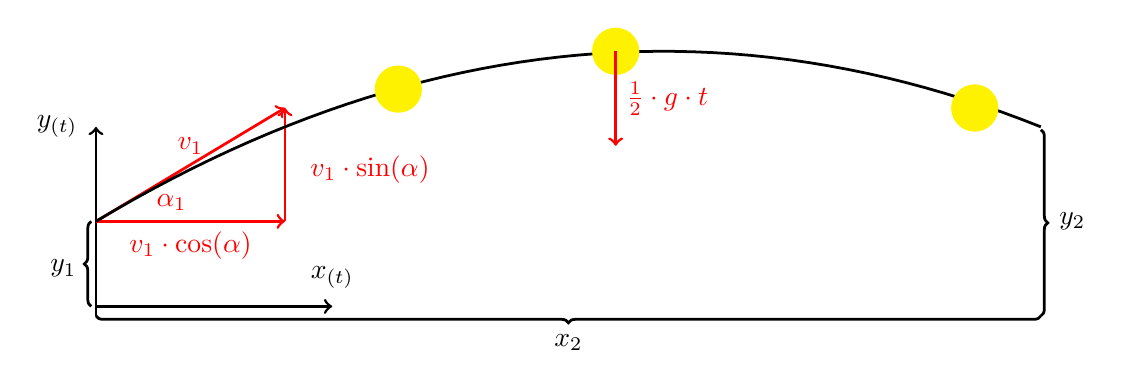
\begin{tikzpicture}[thick,scale=1.2, every node/.style={scale=1}]
        \draw[line width=1pt, decorate, decoration=brace](10, 0) -- (0, 0) (5,0)node 
        [below=1mm]{$x_2$};
        \draw[line width=1pt, decorate, decoration=brace](10, 1.97) -- (10, 0) 
        (10,1) node [right=1mm]{$y_2$};
        \draw[line width=1pt, ->](0, 0) -- (0, 2) node [left=1mm]{$y_{(t)}$};
        \draw[line width=1pt, decorate, decoration=brace](-0.5mm, 1mm) -- 
        (-0.5mm, 1) (3.2mm,0.5) node [left=5mm]{$y_1$};
        \draw[line width=1pt, ->](0, 1mm) -- (2.5, 1mm)  node [above=1mm]{$x_{(t)}$};
        \draw[line width=1pt,red, ->](0, 1) -- node[below]{$v_1 \cdot \cos(\alpha)$} 
        (2, 1);     
        \draw[line width=1pt,red, ->](2, 1) -- (2, 2.2); \node[red] at (2.9,1.55)
        {$v_1 \cdot \sin(\alpha)$}; 
        \draw[line width=1pt,red, ->](0, 1) -- node[above]{$v_1$} (2, 2.2);   
        \draw[line width=1pt,samples=50] plot [domain=0:10](\x,{-1/20*pow(\x-6,2)+2.8});
        \node[red] at (0.8,1.2){$\alpha_1$};
        \fill[yellow] (3.2,2.4) circle (0.25); 
        \fill[yellow] (5.5,2.8) circle (0.25); 
        \fill[yellow] (9.3,2.2) circle (0.25);
        \draw[line width=1pt,red, ->](5.5,2.8) -- node[right]{$\frac{1}{2} \cdot g 
        \cdot t$} (5.5,1.8); 
    \end{tikzpicture}
    \caption{Wurfparabel mit den angreifenden Kräfte}
    \label{fig:WurfparabelKraefte}
\end{figure}

\newpage
\textbf{Berechnungswerte}\\
\begin{tabular}{ll}
    \rule{0pt}{11pt} $\alpha_1$ & $45^\circ$ \\
    \rule{0pt}{11pt} $y_1$ & $0.125 m$ \\
    \rule{0pt}{11pt} $y_2$ & $0.0 m$ \\
    \rule{0pt}{11pt} $x_2$ & $1.8 m$ \\
\end{tabular}\\
\\
\\
\textbf{Resultate}\\
\begin{tabular}{ll}
    \rule{0pt}{11pt} $t$ & $0.56 s$ \\
    \rule{0pt}{11pt} $v_1$ & $4.56 \frac{m}{s}$ \\
\end{tabular}\\
\\
\\
Um den Wurf beurteilen zu können wurde dieser in der Abbildung \ref{fig:Wurfparabel} 
grafisch dargestellt.
\begin{figure}[h!]
    \centering
    \includegraphics[width=1\textwidth,clip,trim=7mm 7mm 7mm 0mm]
    {Enddokumentation/Anhang/Bilder/Schiefer_Wurf.jpg}
    \caption{Wurfparabel}
    \label{fig:Wurfparabel}
\end{figure}\\
%\newpage
Mithilfe der Abwurfgeschwindigkeit kann die Nenndrehzahl durch die Formel 
\ref{equ:v_1} definiert werden.
\begin{equation}  
    n_1 = \frac{v_1}{4\pi \cdot R_s \cdot \cos(\alpha_{Grenz})}
    \label{equ:v_1}
\end{equation}
\newpage
\textbf{Berechnungswerte}\\
\begin{tabular}{ll}
    \rule{0pt}{11pt} $R_s$ & $0.04 m$ \\
    \rule{0pt}{11pt} $\alpha_{Grenz}$ & $16.26^\circ$ \\
    \rule{0pt}{11pt} $v_1$ & $4.56 \frac{m}{s}$ \\
\end{tabular}\\
\\
\\
\textbf{Resultat}\\
\begin{tabular}{ll}
    \rule{0pt}{11pt} $n_1$ & $9.45 \frac{1}{s}$ \\
\end{tabular}\\
\\
Mit den Formeln \ref{equ:Energiegleichung} bis \ref{equ:v_1} kann die Nenndrehzahl gerechnet werden.
\begin{equation}
    m_{Ball} \cdot g \cdot \Delta h + \frac{1}{2} \cdot m_{Ball} \cdot \left[4\pi 
    \cdot R_s \cdot n_1 \cdot \cos(\alpha_{Grenz})\right]^2 + 2 \cdot J \cdot \pi^2 
    \cdot \left(n_1^2-\cdot n_0^2\right) = 0
\end{equation}

\textbf{Berechnungswerte}\\
\begin{tabular}{ll}
    \rule{0pt}{11pt} $m_{ball}$ & $0.055 kg$ \\
    \rule{0pt}{11pt} $g$ & $9.81 \frac{N}{kg}$ \\
    \rule{0pt}{11pt} $\Delta h$ & $0.01465 m$ \\
    \rule{0pt}{11pt} $R_s$ & $0.040 m$ \\
    \rule{0pt}{11pt} $n_1$ & $9.45\frac{1}{s}$ \\
    \rule{0pt}{11pt} $J$ & $0.00018 kgm^2$ \\
    \rule{0pt}{11pt} $\alpha_{Grenz}$ & $16.26^\circ$ \\
\end{tabular}\\
\\
\\
\textbf{Resultat}\\
\begin{tabular}{ll}
    \rule{0pt}{11pt} $n_0$ & $15.89 \frac{1}{s}$ \\
\end{tabular}\\
\begin{equation}
    \frac{n_1}{n_0} = 0.4 \label{equ_Prozentwert}
\end{equation}
Bei dem zurzeit vorhandenen Trägheitsmoment (Vollwelle) wird die Drehzahl um 40\% 
abgebremst. Die dabei verlorene Energie muss vom Motor zugeführt werden. 
Die Zeitdauer dafür berechnet sich wie folgt.
\begin{align}
    M_{Motor} &= \omega \cdot J \\
    n_0 &= n_1 + \omega \cdot t \\
    t &= \frac{n_0 - n_1}{\omega} = \frac{J \cdot \left(n_0 - n_1\right)}{M_{Motor}}
\end{align}

\textbf{Berechnungswerte}\\
\begin{tabular}{ll}
    \rule{0pt}{11pt} $n_0$ & $15.89 \frac{1}{s}$ \\
    \rule{0pt}{11pt} $n_1$ & $9.45 \frac{1}{s}$ \\
    \rule{0pt}{11pt} $J$ & $0.00018 kgm^2$ \\
    \rule{0pt}{11pt} $M$ & $0.1 Nm$ \\
\end{tabular}\\
\\
\\
\textbf{Resultat}\\
\begin{tabular}{ll}
    \rule{0pt}{11pt} $t$ & $0.0116 s$ \\
\end{tabular}\\
\\
Fazit dieser Berechnungen ist, dass ein erhöhtes Trägheitsmoment, die Schwungräder 
weniger abbremst, und ein grösseres Drehmoment diese schneller wieder auf die 
Nenndrehzahl beschleunigt. 

            \newpage
            \subsubsection{Berechnung Drehmoment Förderband}
Für die Berechnungen werden verschiedene Formelzeichen verwendet, die in 
der Tabelle \ref{tab:glossarFoerderband} aufgeführt und deren Bedeutung erklärt sind.
\begin{table}[h!]
    \begin{tabular}{lcl}
    \rule{0pt}{11pt}Zeichen & Einheit & Bezeichnung \\
    \hline\rule{0pt}{11pt} $M_{Motor}$ & $Nm$ & Drehmoment Motor \\
    \rule{0pt}{11pt}$M_{Antrieb}$ & $Nm$ & Drehmoment an der Antriebstrommel \\
    \rule{0pt}{11pt}$i$ & $1$ & Übersetzungsverhältnis \\
	\rule{0pt}{11pt}$z_1$ & $1$ & Zähnezahl getriebenes Rad \\
	\rule{0pt}{11pt}$z_2$ & $1$ & Zähnezahl Ritzel \\
	\rule{0pt}{11pt}$F_u$ & $N$ & Umfangskraft an Antriebstrommel \\
	\rule{0pt}{11pt}$r_A$ & $m$ & Radius der Antriebstrommel \\
	\rule{0pt}{11pt}$\mu$ & $1$ & Haftreibungskoeffizient Band zu Auflagefläche \\
	\rule{0pt}{11pt}$g$ & $\frac{N}{kg}$ & Erdbeschleunigung \\
	\rule{0pt}{11pt}$m_{Ball}$ & $kg$ & Masse des Balles \\
	\rule{0pt}{11pt}$m_{Umlenkrolle}$ & $kg$ & Masse der Umlenkrolle \\
	\rule{0pt}{11pt}$m_{Band}$ & $kg$ & Masse des Bandes \\
	\rule{0pt}{11pt}$v_{Band}$ & $\frac{m}{s}$ & Geschwindigkeit des Bandes \\
	\rule{0pt}{11pt}$n_{Motor}$ & $\frac{1}{s}$ & Drehzahl Motor \\
    \end{tabular}
	\centering
	\caption{Glossar für die Berechnung des Förderbandes}
	\label{tab:glossarFoerderband}
\end{table}

Um einen geeigneten Antrieb für das Förderband zu erörtern, muss das Drehmoment 
und die Drehzahl bekannt sein.
\begin{figure}[h!]
    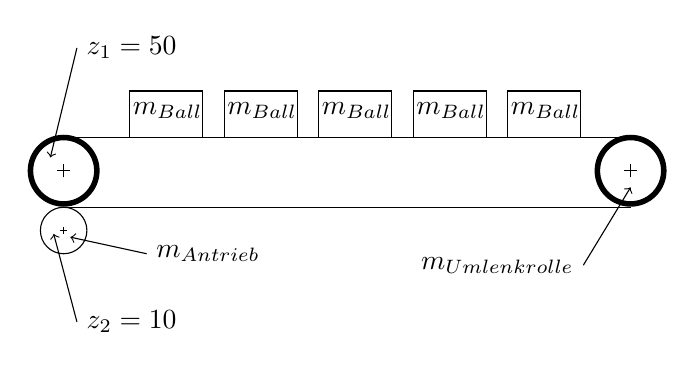
\begin{tikzpicture}[scale = 1.2]
        \draw [-,line width=2pt](0,0) circle (10pt);\draw [-,line width=2pt](6,0) circle (10pt); 
        %beide Kreise der Hauptrollen
        \draw  (0,10pt) -- (6, 10pt); \draw (0,-11pt) -- (6,-11pt); %die beiden Förderbänder-Striche
        \draw (0,-2pt) -- (0, 2pt); \draw (0cm-2pt,0) -- (0cm+2pt, 0); %Das x der ersten Rolle
        \draw (6,-2pt) -- (6, 2pt); \draw (6cm-2pt,0) -- (6cm+2pt, 0); %Das x der zweiten Rolle
        \draw [<-] (6cm-0pt , -5pt) -- (5.5,-1)node[left]{$m_{Umlenkrolle}$}; %zeige-Linie auf das 
        %Hintere Rad mit Text
        \draw (0.7,10pt) -- ++(0, 14pt)-- ++(22pt,0) -- ++(0, -14pt);\node  at (1.1,18pt) {$m_{Ball}$};
        \draw (1.7,10pt) -- ++(0, 14pt)-- ++(22pt,0) -- ++(0, -14pt);\node  at (2.1,18pt) {$m_{Ball}$};
        \draw (2.7,10pt) -- ++(0, 14pt)-- ++(22pt,0) -- ++(0, -14pt);\node  at (3.1,18pt) {$m_{Ball}$};
        \draw (3.7,10pt) -- ++(0, 14pt)-- ++(22pt,0) -- ++(0, -14pt);\node  at (4.1,18pt) {$m_{Ball}$};
        \draw (4.7,10pt) -- ++(0, 14pt)-- ++(22pt,0) -- ++(0, -14pt);\node  at (5.1,18pt) {$m_{Ball}$};
        \draw (0,-18pt) circle (7pt);  \draw [<-] (2pt , -20pt) -- (25pt,-25pt)node[right]
        {$m_{Antrieb}$}; %zeige-Linie auf das Antriebsrad mit Beschriftung
        \draw (-1pt,-18pt) -- (1pt,-18pt); \draw (0,-19pt) -- (0, -17pt); %Das x der zweiten Rolle
        \draw [<-] (-4pt , 4pt) -- (4pt,1.3)node[right]{$z_1 = 50$}; %zeige-Linie auf das linke 
        %Umlenkrad mit Beschriftung
        \draw [<-] (-3pt , -19pt) -- (4pt,-1.6)node[right]{$z_2 = 10$}; %zeige-Linie auf das 
        %Antriebsrad mit Beschriftung
    \end{tikzpicture}
   	\centering
    \caption{Erläuterungen zur Förderbandberechnung}
\end{figure}
\begin{align}
    M_{Motor} &= M_{Antrieb} \cdot i \label{equ:M_Antrieb}\\
    i &=\frac{z_1}{z_2}\\
    M_{Antrieb} &= F_u \cdot r_A\\
    F_u &= \mu \cdot g \cdot \left(5 \cdot m_{Ball} + m_{Umlenkrolle} + m_{Band} \right)\label{equ:F_u}
\end{align}
\\
Aus den Formeln \ref{equ:M_Antrieb} bis \ref{equ:F_u} ergibt dies benötigte Drehmoment am Motor. 
\begin{align}
    M_{Motor} &= \mu \cdot g \cdot r_A \cdot \left(5 \cdot m_{Ball} + m_{Umlenkrolle} + m_{Band}\right) 
    \cdot \frac{z_1}{z_2} \\
    n_{Motor} &=\frac{v_{Band}}{2 \cdot r_A \cdot \pi} \cdot i
\end{align}

\textbf{Berechnungswerte}\\
\begin{tabular}{lll}
	\rule{0pt}{11pt} $g$ & $9.81 \frac{N}{kg}$ & \\
	\rule{0pt}{11pt} $m_{ball}$ & $0.055 kg$ & \\
	\rule{0pt}{11pt} $m_{Umlenkrolle}$ & $0.020 kg$ & gemäss CAD \\
	\rule{0pt}{11pt} $m_{Band}$ & $0.035 kg$ & gemäss Datenblatt \\
	\rule{0pt}{11pt} $z_1$ & $50$ & gewählte Übersetzung \\
	\rule{0pt}{11pt} $z_2$ & $10$ & gewählte Übersetzung \\
	\rule{0pt}{11pt} $r_a$ & $0.020 m$ & gemäss Konstruktion \\
	\rule{0pt}{11pt} $v_{Band}$ & $0.1 \frac{m}{s}$ & vorgegebener Wert \\
\end{tabular}\\
\\
\\
\textbf{Resultate}\\
\begin{tabular}{ll}
	\rule{0pt}{11pt} $M_{motor}$ & $0.0987 Nm$ \\
	\rule{0pt}{11pt} $n_{motor}$ & $3.98 \frac{1}{s}$ \\
\end{tabular}
            \newpage
            \subsubsection{Berechnung Horizontale Ausrichtung}
Für die Stelleinheit wird ein Schrittmotor eingesetzt. Der Antriebsstrang muss 
hinsichtlich Drehmoments ausgelegt werden. Die Antriebsritzel wurden so gewählt, 
dass ein möglichst leichter Schrittmotor verwendet werden kann. 
\begin{align}
    F_{Losteil} &= m_{Losteil} \cdot g\\
    F_2 &= F_{Losteil} \cdot 0.1
\end{align}
\begin{align}
    M_{Drehung} &= L \cdot F_{2R}\\
    F_{2R} &= \mu_H \cdot F_2
\end{align}
\begin{align}
    M_{Motor} &= F_z \cdot r\\
    F_z &= \frac{M_{Drehung}}{R}\\
    M_{Motor} &=\frac{L \cdot \mu_H \cdot m_{Losteil} \cdot g \cdot 0.1}{R} \cdot r
\end{align}

\textbf{Berechnungswerte}\\
\begin{tabular}{lll}
	\rule{0pt}{11pt} $m_{Losteil}$ & $1.6 kg$ & \\
	\rule{0pt}{11pt} $g$ & $9.81 \frac{N}{kg}$ & \\
	\rule{0pt}{11pt} $L$ & $0.437 m$ &  \\
	\rule{0pt}{11pt} $\mu_H$ & $0.2$ & Haftreibungskoeffizient zwischen Rolle und Boden \\
	\rule{0pt}{11pt} $r$ & $0.01 m$ & \\
	\rule{0pt}{11pt} $R$ & $0.28 m$ & \\
\end{tabular}\\
\\
\\
\textbf{Resultate}\\
\begin{tabular}{ll}
	\rule{0pt}{11pt} $M_{motor}$ & $0.0049Nm$ \\
\end{tabular}
    		\newpage
		\includepdf[page=1 , offset=0cm -1.9cm,frame, width=0.94\textwidth,picturecommand={\centering},pagecommand=\subsection{Stepper-Dokumentation}\label{Stepper_Dokumentation}{\thispagestyle{fancy}},]{Enddokumentation/Anhang/Extern/Stepper_StandaloneDoc.pdf}

%pagecommand=\section{Projektplan}
\includepdf[page=2- , offset=0cm -1.35cm,frame, width=\textwidth,picturecommand={\centering},pagecommand={\thispagestyle{fancy}},]{Enddokumentation/Anhang/Extern/Stepper_StandaloneDoc.pdf}
	\end{appendix}  
\end{document}